\chapter{Uvod}

Zaštita elektroenergetskih sistema danas je jako aktuelan i bitan problem koji se nameće u radu elektroenergetskih sistema. Potrebno je u slučaju kvara pravovremeno reagovati kako bi se ograničila moguća šteta opreme, ali i smanjila ili potpuno eliminisala opasnost za ljude. Cilj je što je više moguće reducirati utjecaj kvara na sistem.

\section{Distantna zaštita}

Neke od najznačanijih tipova zaštita elektroenergetskih sistema su:

\begin{itemize}
    \item diferencijalna zaštita
    \item \textbf{distantna zaštita}
    \item prekostrujna zaštita
    \item pod/preko naponska zaštita
    \item pod/preko frekventna zaštita... \cite{prva}
\end{itemize}

Porast potražnje električne energije vodi ka širenju i
usložnjavanju elektroenergetskog sistema za distribuciju električne energije, što postavlja sve složenije zahtjeve na projekovanje i podešenje sistema relejne zaštite. Primjenom prekostrujnih i usmjerenih prekostrujnih zaštita ne postiže se zadovoljavajuća selektivnost i brzina djelovanja, pa se složene distributivne mreže danas uglavnom štite distantnim relejima. Moderni numerički digitalni uređaji relejne zaštite obično imaju u sebi ugrađenu mogućnost djelovanja i kao prekostrujni i kao distantni relej, pa to olakšava zaštitu. \cite{druga} Oznaka za distantni relej po standardu ANSI/IEEE C37.2 je \textbf{21}.

U mrežama koje koriste više izvora napajanja što ih čini složenijim, kao i u prijenosim mrežama, primarna zaštita dugih vodova je isključivo distantna zaštita. Distantna zaštita je univerzalna zaštita od kratkih spojeva, posebno u visokonaponskim prijenosnim mrežama sa direktno uzemljenom neutralnom tačkom. Još neke od njenih primjena koje se rjeđe koriste su, kao što je spomenuto, primjene u distributivnim mrežama i kao rezervna zaštita velikih energetskih transformatora i generatora (eng. \textbf{G}enerator \textbf{S}tep-\textbf{U}p transformers - GSU blok). \cite{prva}

Distantni relej ima dva ulaza: napon i struju na mjestu na vodu gdje se nalazi relej. Idealni distantni relej ne ovisi o veličinama napona i struje pojedinačno već samo o njihovom omjeru i faznom uglu između njih. \cite{druga} Kako se distantna zaštita koristi uglavnom za zaštitu linija, u nastavku će biti predstavljena upravo ovakva zaštita. \cite{prva} Od distantne zaštite možemo izvući tri krucijalne informacije:

\begin{itemize}
    \item da se desio kvar
    \item koji se kvar desio
    \item lokaciju kvara.
\end{itemize}

Koristeći fazore napona i struje, relej računa impedansu te je uspoređuje sa parametrima linije koji su poznati. Linija je predstavljena svojim $\pi$ ekvivalentom. Šema primjera zaštite jedne linije prikazana je slikom \ref{fig:slika1} na kojoj je prikazano i predstavljanje linije preko njenog $\pi$ ekvivalenta. Slikom \ref{fig:shema2} prikazano je simbolički uspostavljanje ravnoteže, tj. možemo postaviti uslove ravnoteže:
 \[ f_0(U_F)=kf_1(I_F)\]
odnosno:
\[k=\frac{U_F}{I_F}=Z_F\]


\begin{figure}[H]
  \centering
  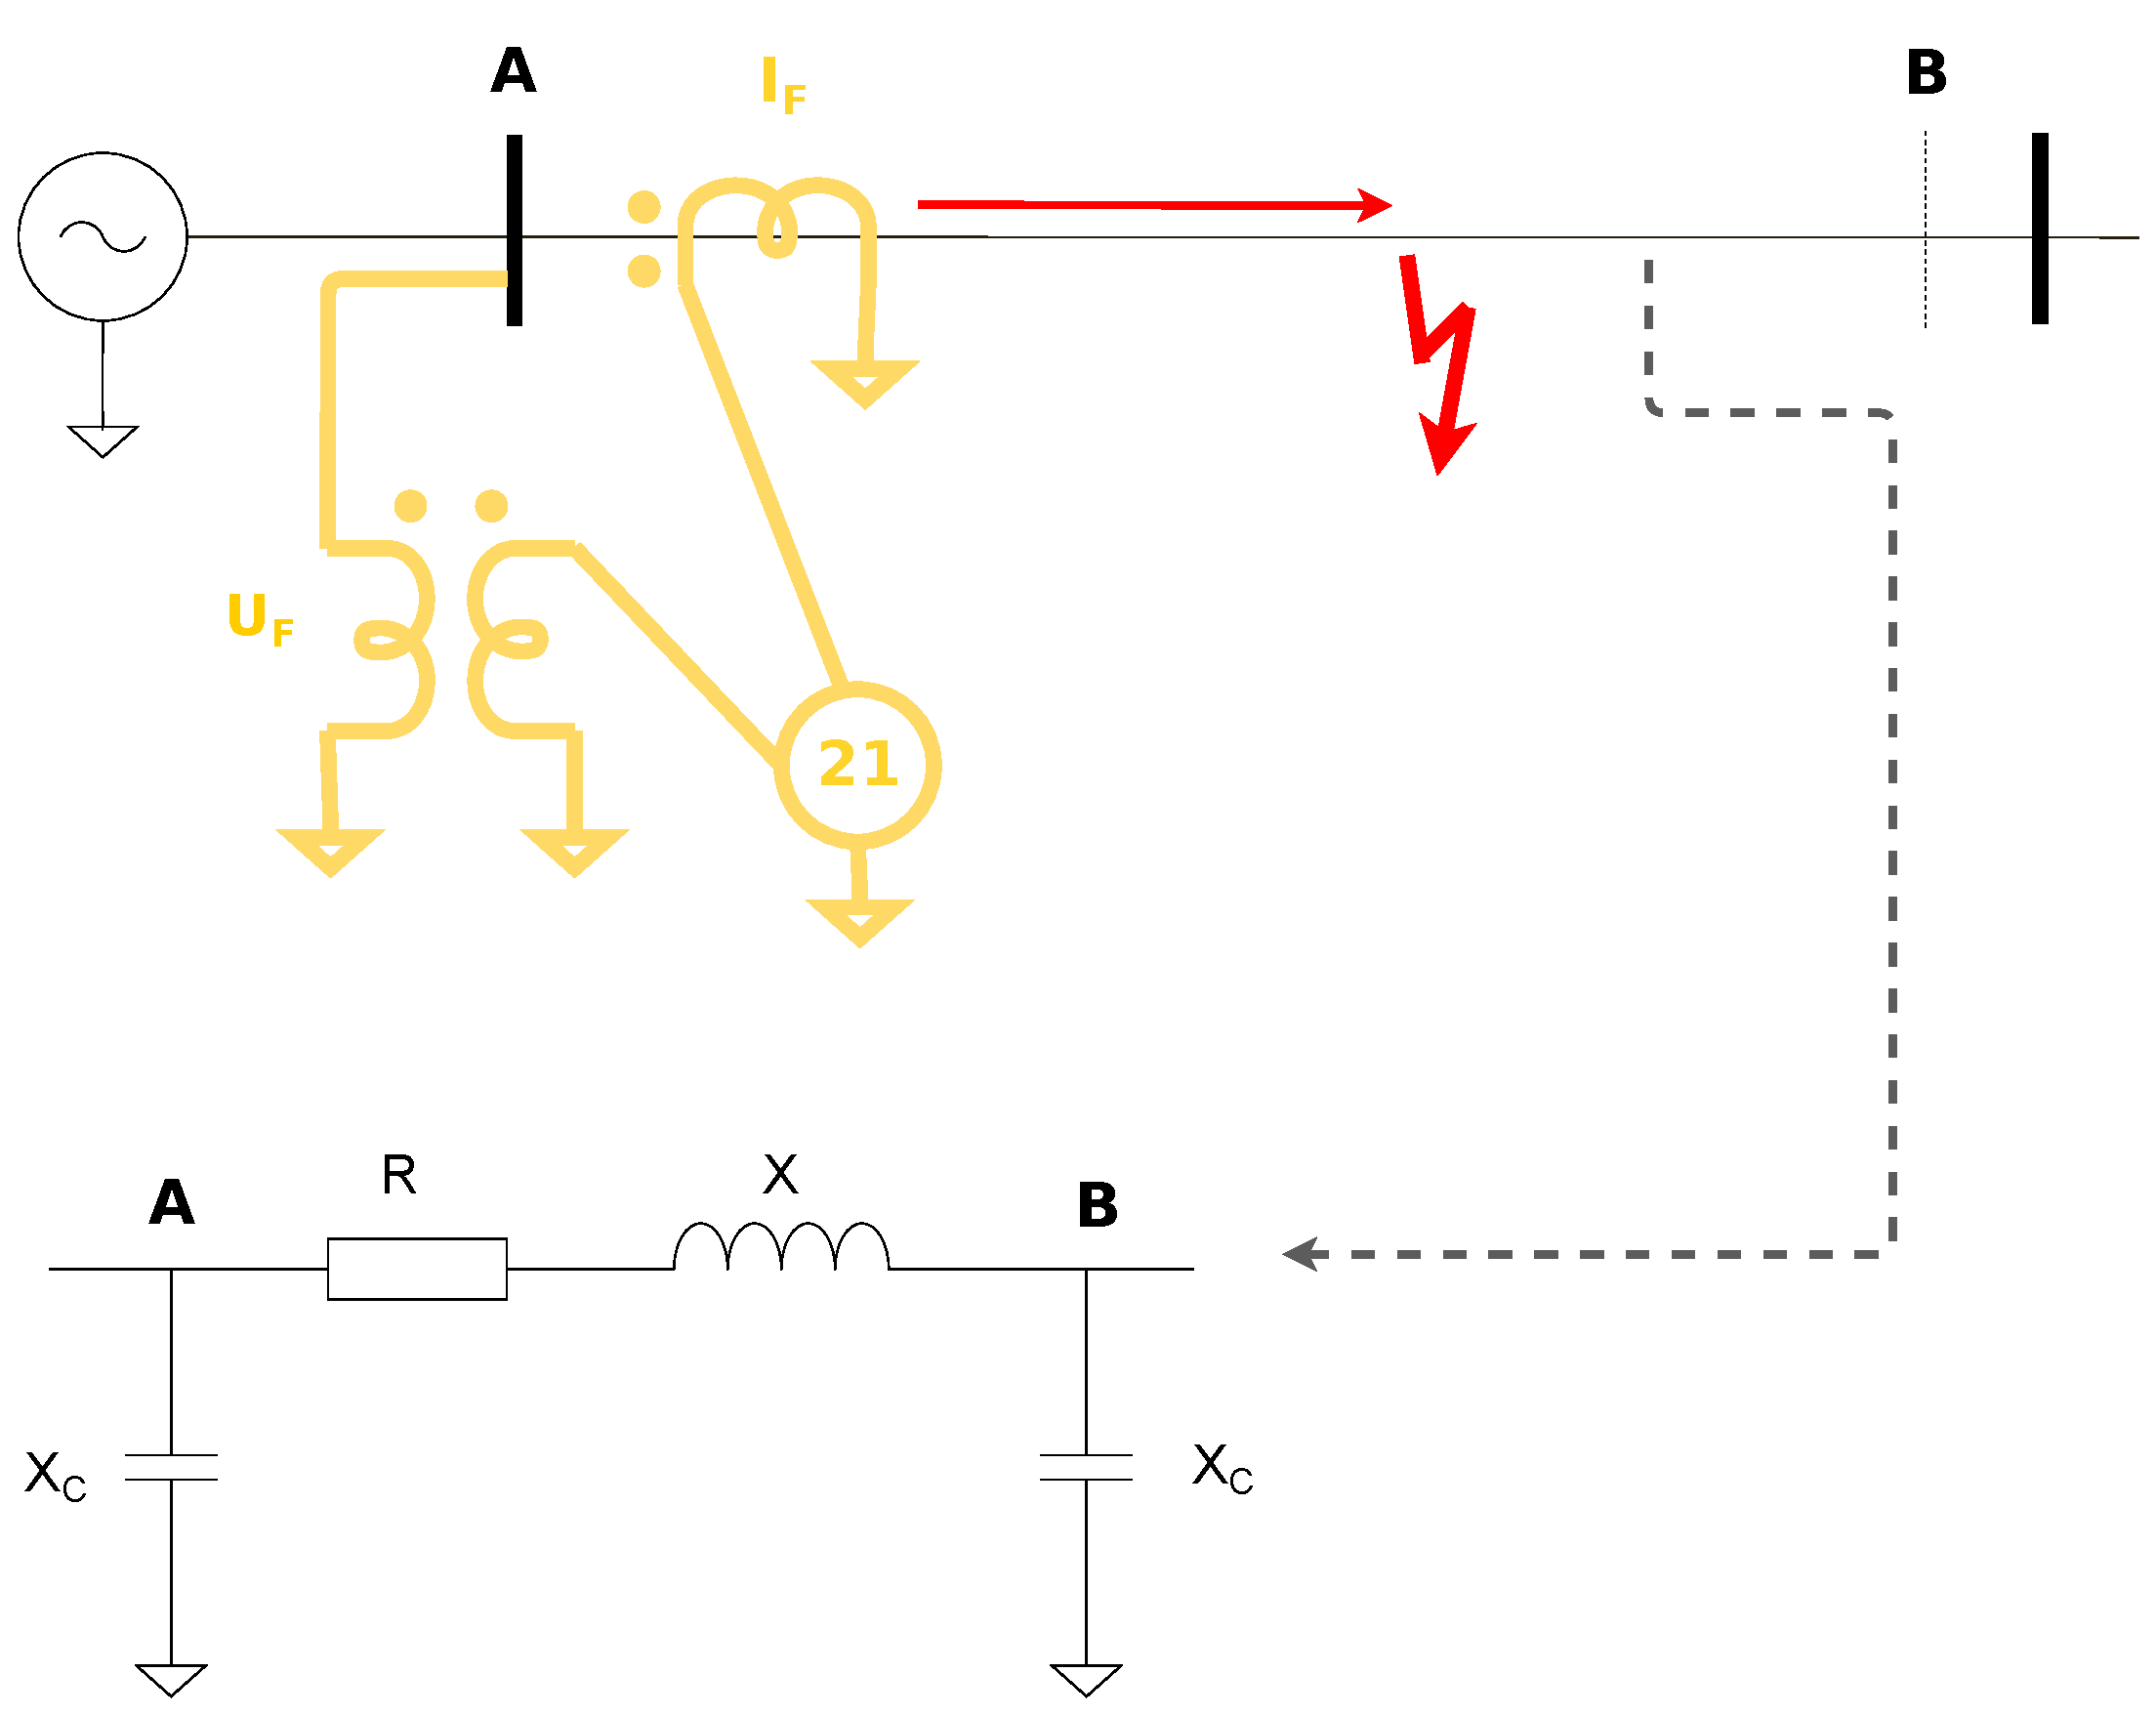
\includegraphics[width=0.8\textwidth]{shema1}
  \caption{Distantna zaštita linije}
  \label{fig:shema1}
\end{figure}

\begin{figure}[H]
  \centering
  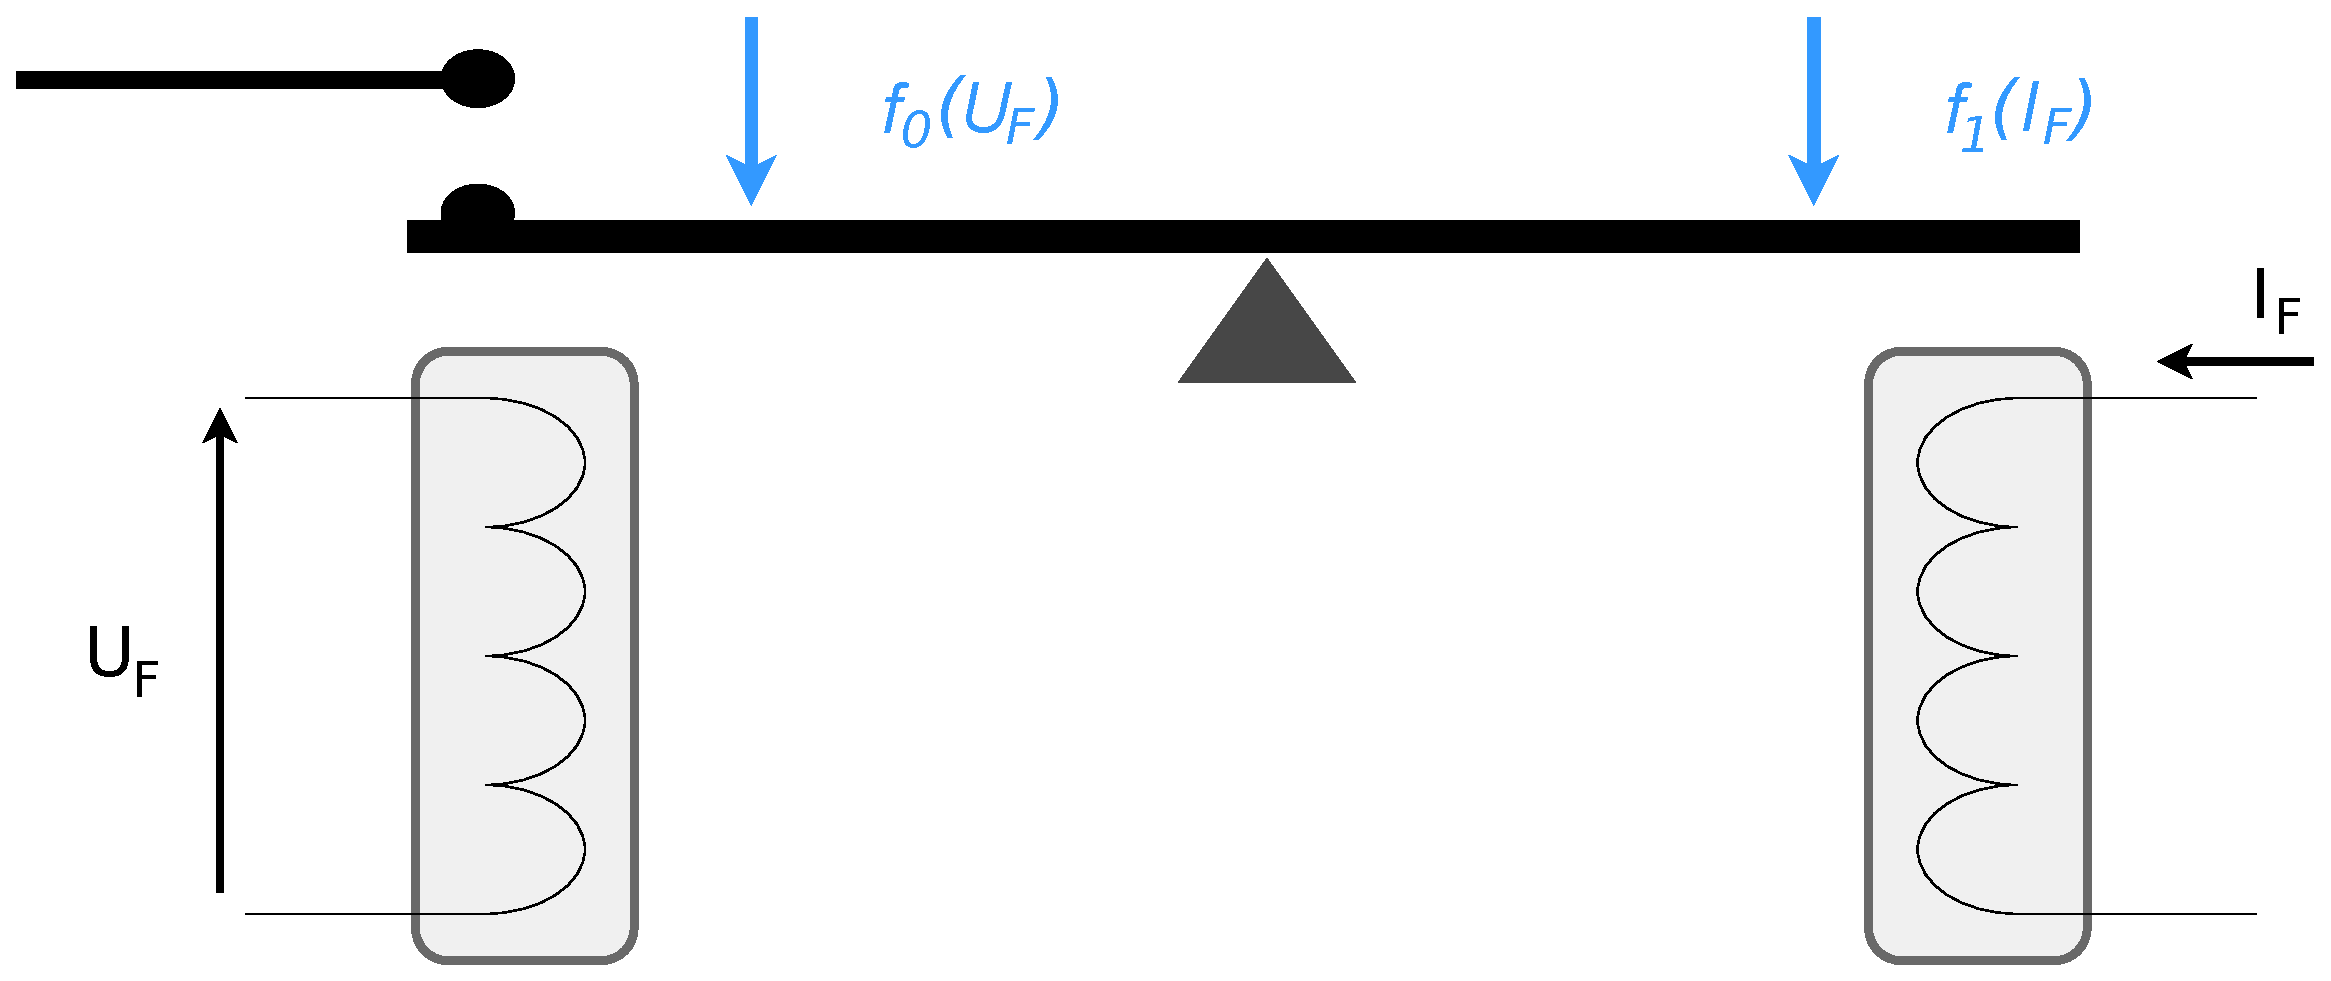
\includegraphics[width=0.7\textwidth]{shema2}
  \caption{Uslov ravnoteže}
  \label{fig:shema2}
\end{figure}

Kao što je rečeno, koristeći fazore napona i struje, relej računa impedansu te je upoređuje sa parametrima linije. Uzimajući u obzir da se radi o trofaznom sistemu, dobivamo tri fazna napona i tri fazne struje koje se koriste na sličan način:

\begin{itemize}
    \item računaju se tri impedanse za petlje između svake faze ($Z_{ab}, Z_{bc}, Z_{ca}$)
    \item računaju se tri impedanse za petlje između svake faze i zemlje ($Z_{ag}, Z_{bg}, Z_{cg}$)
    \item ukoliko se bilo koja od izračunatih impedansi nalazi unutar proradnog područja karakteristike releja, relej će proraditi. 
\end{itemize}

Proradna karakteristika crta se u ${R, X}$ ravni. O proradnim karakteristikama bit će nešto više rečeno kasnije.

Posmatrajmo simetričnu liniju za koju je serijska grana definisana sa matricom impedansi:

\[Z_{abc}=\begin{pmatrix} z_{aa} & z_{ab} & z_{ac} \\
z_{ba} & z_{bb} & z_{bc} \\
z_{ca} & z_{cb} & z_{cc} \end{pmatrix} = \begin{pmatrix}  z_{s} & z_{m} & z_{m} \\
z_{m} & z_{s} & z_{m} \\
z_{m} & z_{m} & z_{s} \end{pmatrix}\]

za koju važi $U_{abc}=Z_{abc}I_{abc}$, a ukoliko struje i napone prebacimo u sistm simetričnih komponenti $012$ imamo:

\[T^{-1}U_{012}=Z_{abc}T^{-1}I_{012}\] 

tj. ukoliko pomnožimo s lijeve strane prethodnu jednačinu sa $T$ dobijemo:

\[U_{012}=TZ_{abc}T^{-1}I_{012}\]

te nakon toga možemo napisati da je:

\[Z_{012}=TZ_{abc}T^{-1}=\begin{pmatrix} z_{0} & 0 & 0 \\
0 & z_{1} & 0 \\
0 & 0 & z_{2} \end{pmatrix} = \begin{pmatrix}  z_{0} & 0 & 0 \\
0 & z_{1} & 0 \\
0 & 0 & z_{1} \end{pmatrix}\]

gdje je:

\[T=\frac{1}{3} \begin{pmatrix} 1 & 1 & 1 \\
1 & a & a^2 \\
1 & a^2 & a \end{pmatrix}\]

\[a=cos(\frac{2\pi}{3})+jsin(\frac{2\pi}{3})\] 

Kako bismo objasnili princip rada distantne zaštite, izvest ćemo proračun impedansi za dvofazni kratak spoj. Uzmimo primjer da se desio kratki spoj između faza b i c. Ovakav slučaj prikazan je slikom \ref{fig:shema3} odakle možemo vidjeti da vrijedi:

\[\begin{pmatrix} I_a \\ I_b \\ I_c \end{pmatrix}=\begin{pmatrix} 0 \\ I_f \\ -I_f \end{pmatrix}\]

te

\[U_{b_{f}}=U_{c_{f}}\]

\begin{figure}[H]
  \centering
  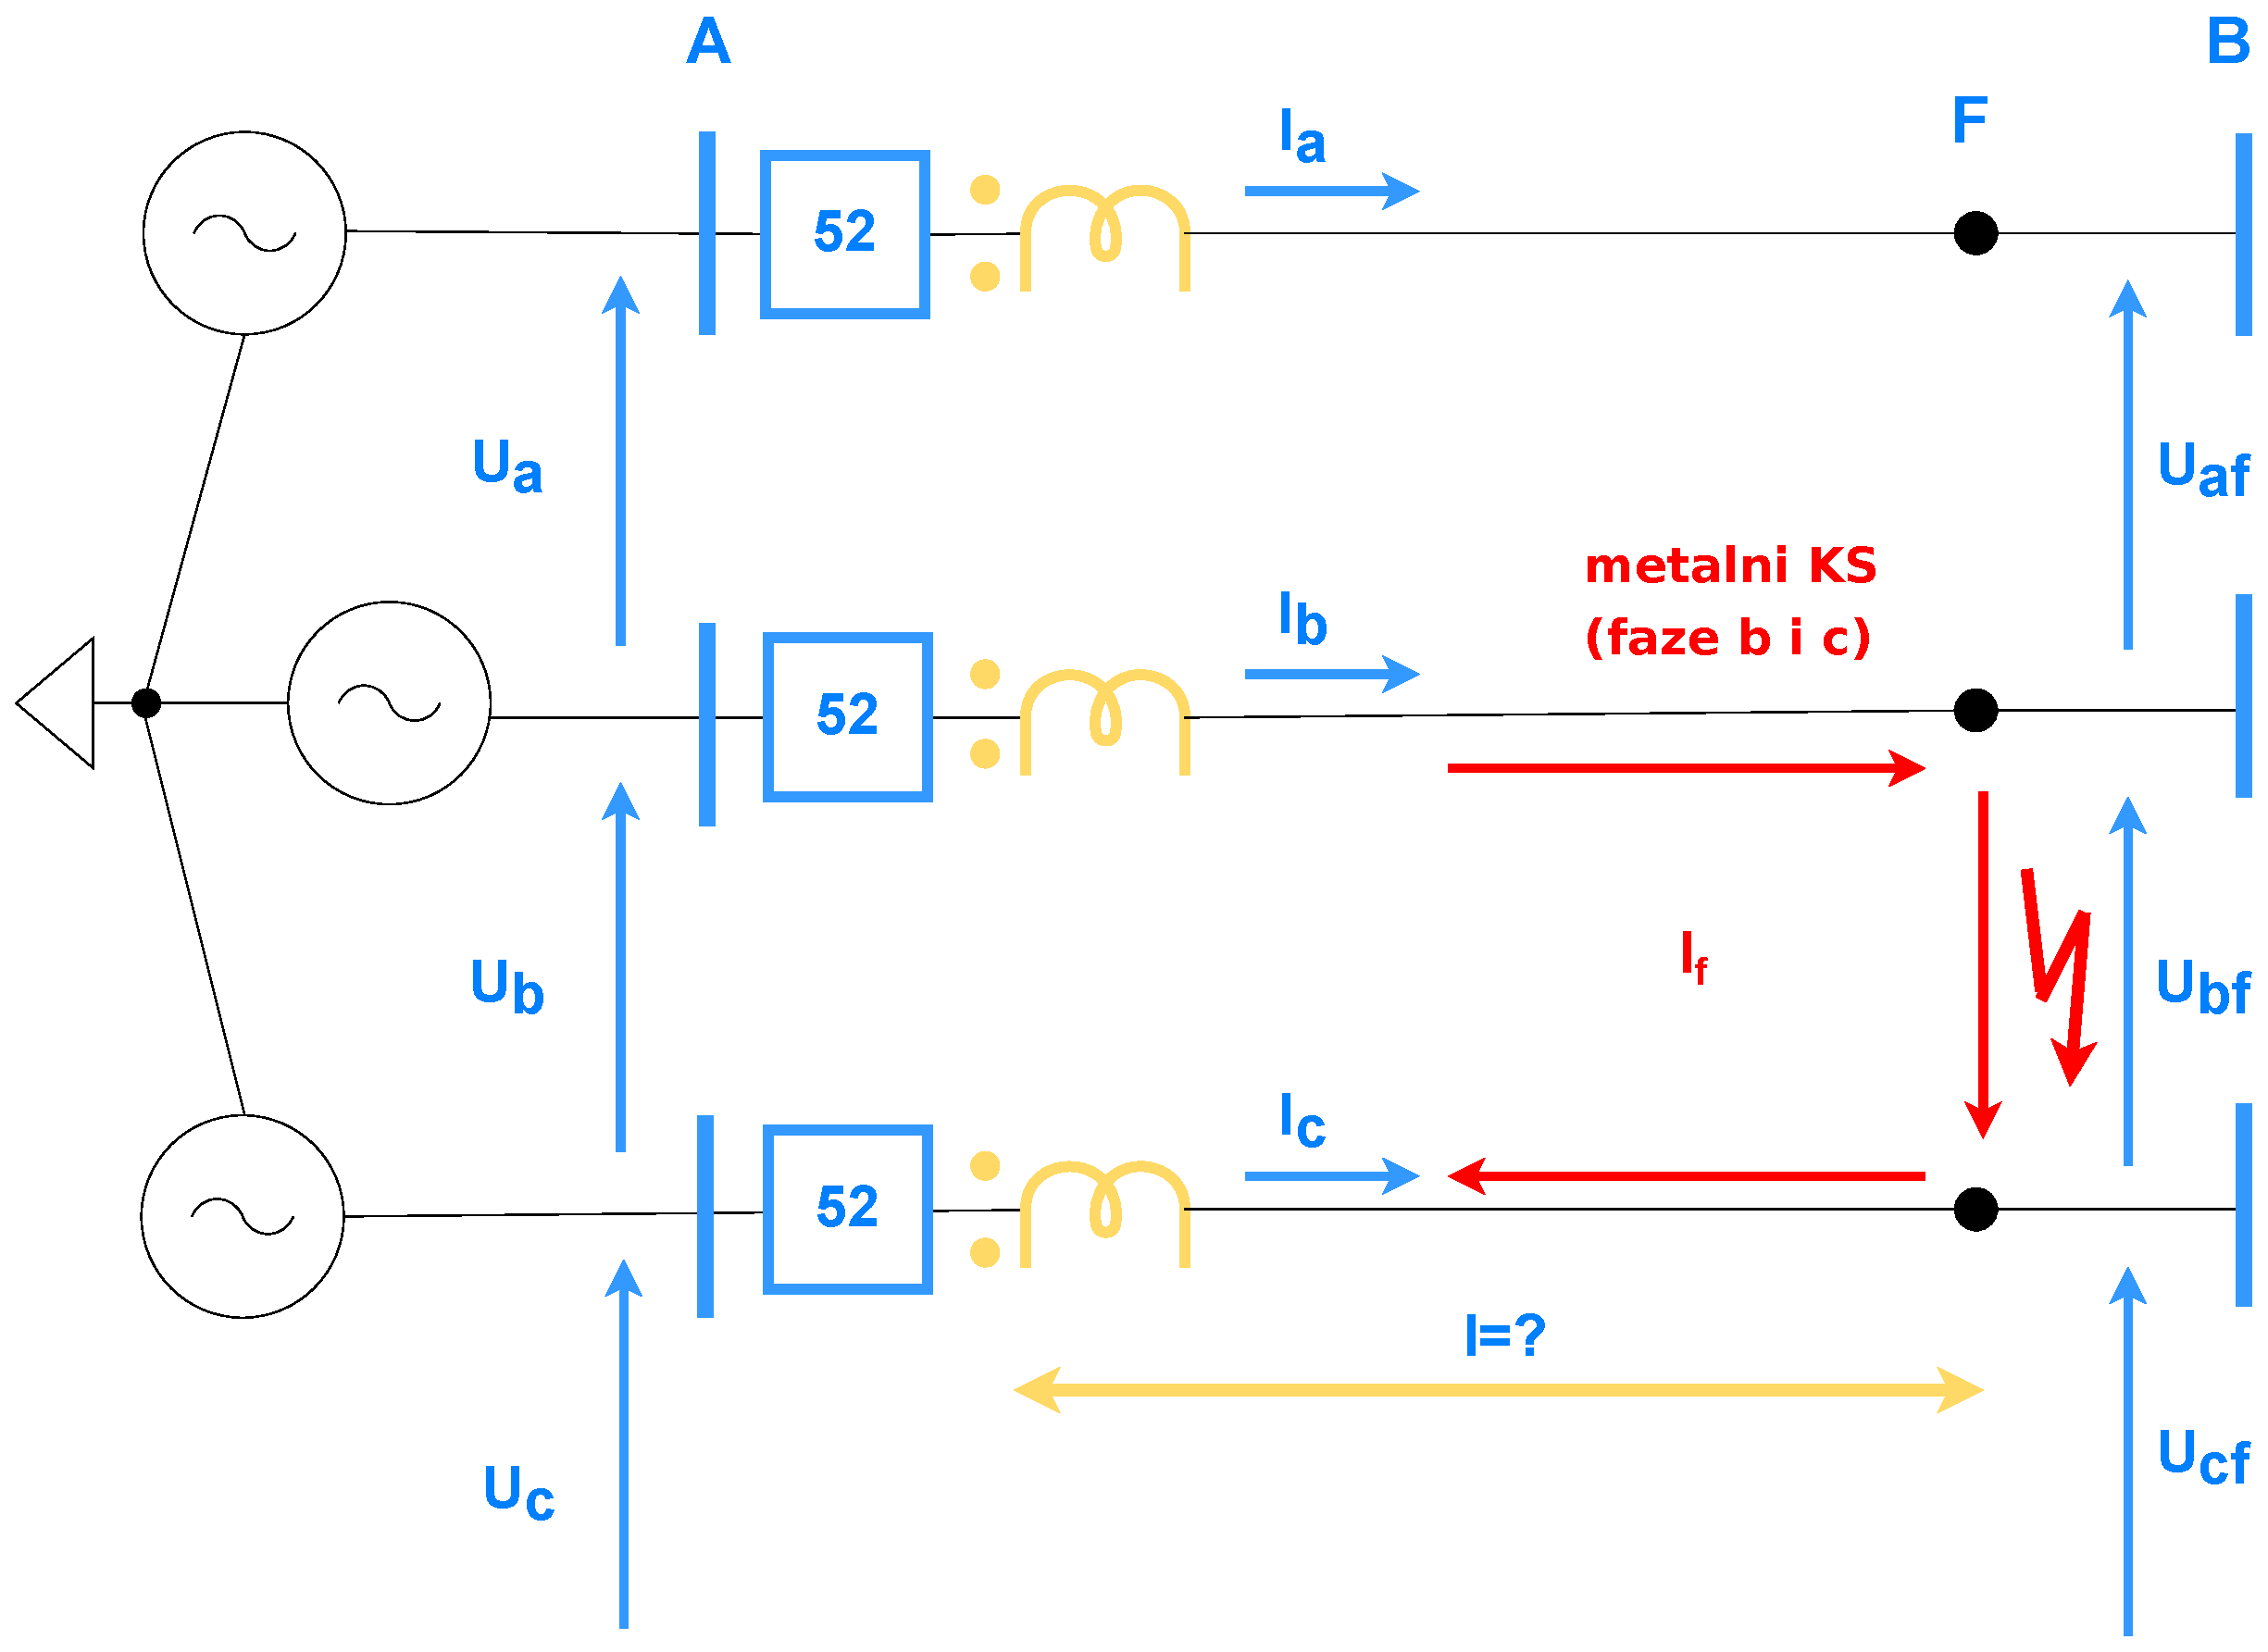
\includegraphics[width=1\textwidth]{shema3}
  \caption{Kratki spoj faza b i c}
  \label{fig:shema3}
\end{figure}

Ako sada struje prebcimo u simetrične komponente, imat ćemo:

\[I_{012}=TI_{abc}=\frac{1}{3} \begin{pmatrix} 0+I_f-I_f \\ 
0+aI_f-a^2I_f \\
0+a^2I_f-aI_f \end{pmatrix}=\frac{1}{3} \begin{pmatrix} 0 \\
aI_f-a^2I_f \\
-(aI_f-a^2I_f) \end{pmatrix}=\begin{pmatrix} 0 \\
I_1 \\
I_2 \end{pmatrix} \]

Iz prethodnih jednačina možemo zaključiti da ne postoji nulta komponenta u slučaju dvofaznog kratkog spoja i da je $I_1=-I_2$.

Pretvarajući napone u simetrične komponente:

\[U_{012}=TU_{abc}=T \begin{pmatrix} U_{a_{f}} \\
U_{b_{f}} \\
U_{b_{f}} \end{pmatrix}=\frac{1}{3} \begin{pmatrix} U_{a_{f}}+U_{b_{f}}+U_{b_{f}} \\
U_{a_{f}}+aU_{b_{f}}+a^2U_{b_{f}} \\
U_{a_{f}}+a^2U_{b_{f}}+aU_{b_{f}} \end{pmatrix}=\frac{1}{3} \begin{pmatrix} U_{a_{f}}+U_{b_{f}}+U_{b_{f}} \\
U_{a_{f}}+U_x \\
U_{a_{f}}+U_x \end{pmatrix}=\begin{pmatrix} U_0 \\
U_1 \\
U_2 \end{pmatrix} \]

vidimo da je $U_1=U_2$, te uzimajući da je $I_1=-I_2$ možemo zaključiti da se ovo postiže samo ukoliko su pozitivna i negativna komponenta spojene paralelno. 

Slikom \ref{fig:shema4} je prikazan model dvofaznog kvara preko simetričnih komponenti (nulta, pozitivna i negativna), tj. njihovog Theveninovog ekvivalenta i ostatka linije.

\begin{figure}[H]
  \centering
  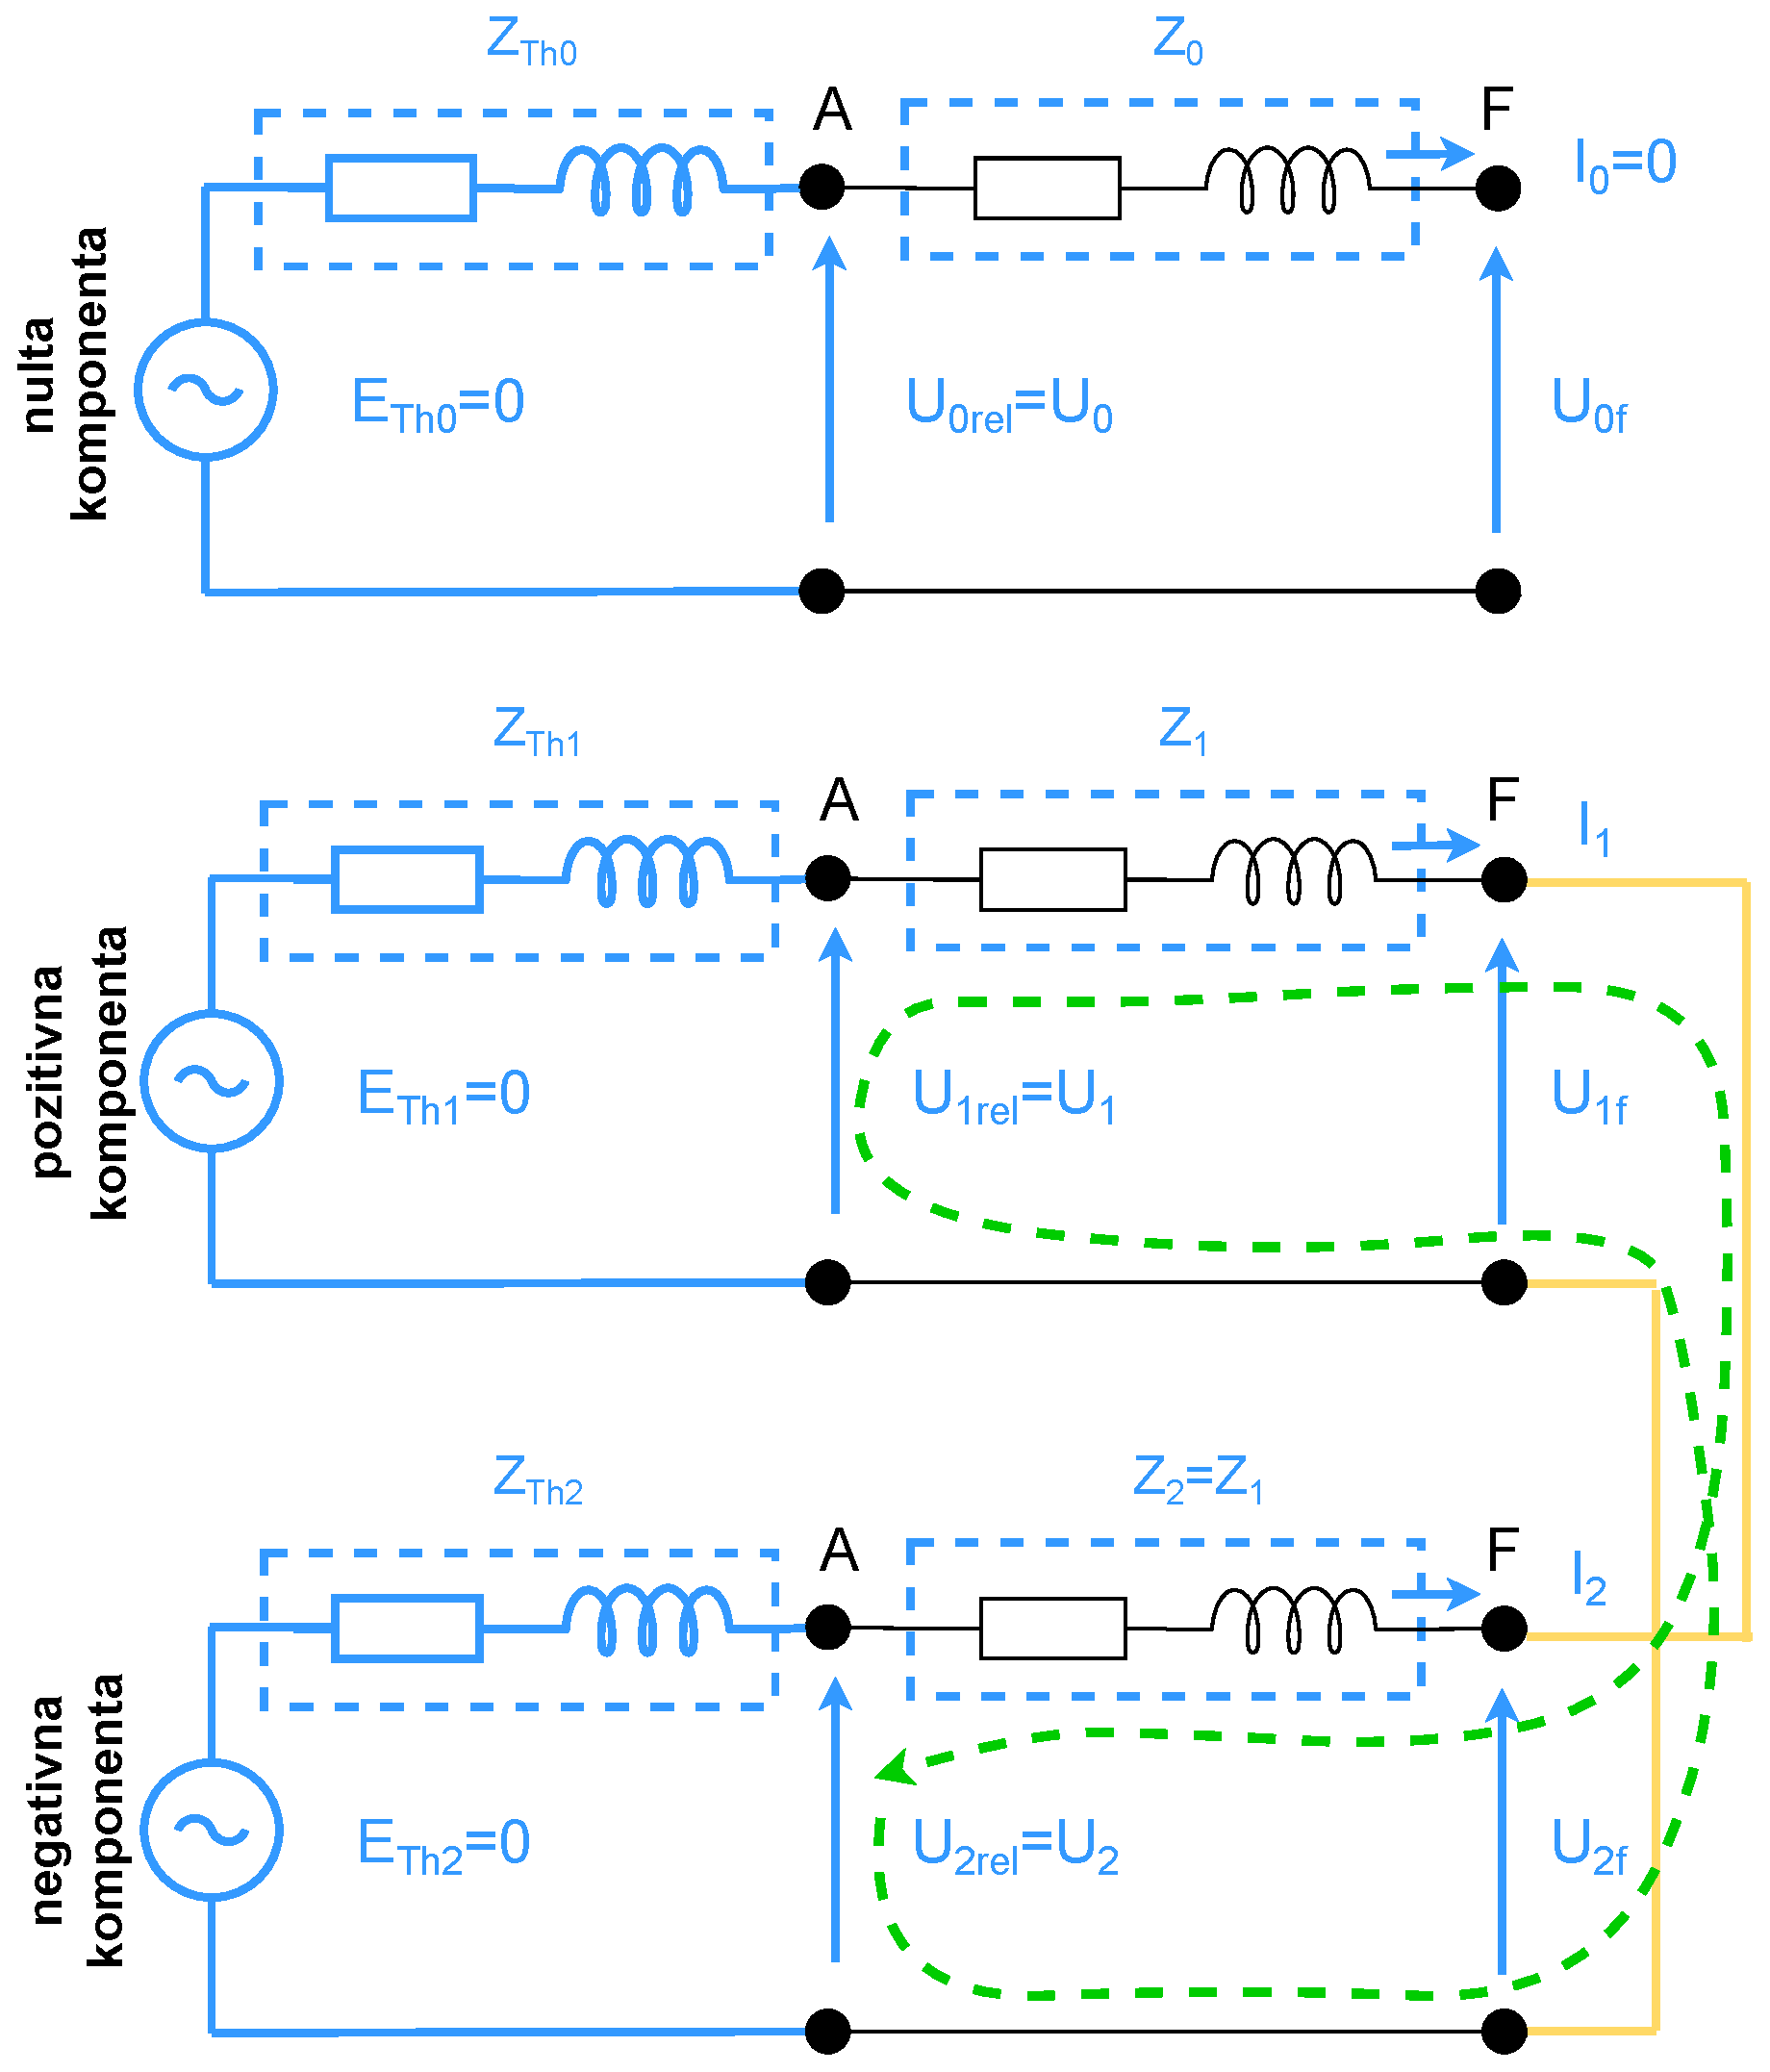
\includegraphics[width=0.9\textwidth]{shema4}
  \caption{Model dvofaznog kratkog spoja prikazan preko simetričnih komponenti}
  \label{fig:shema4}
\end{figure}

Postavljajući Kirchhoffov zakon za napone u petlji koja je naznačena između pozitivne i negativne komponente i uz uslov da je $Z_2=Z_1$ imamo da je:

\[U_2-Z_1I_2+Z_1+Z_1I_1-U_1=0\]
\[Z_1(I_1-I_2)=U_1-U_2\]
tj.
\[Z_1=\frac{U_1-U_2}{I_1-I_2} (*)\]

U sistemu nesimetričnih komponenti vrijedi:

\[U_{abc}=T^{-1}U_{012}=\begin{pmatrix} 1 & 1 & 1 \\
1 & a^2 & a \\
1 & a & a^2 \end{pmatrix} \begin{pmatrix} U_0 \\
U_1 \\
U_2 \end{pmatrix} \]

odakle se izvodi da je:

\[U_1-U_2=\frac{U_b-U_c}{a^2-a} (**) \]

Također se na sličan način iz veze struja simetričnih i nesimetričnih komponenti može pokazati da je:

\[I_1-I_2=\frac{I_a-I_b}{a^2-a} (***) \]

Ukoliko uvrstimo (**) i (***) u (*) dobivamo:

\[Z_1=\frac{U_b-U_c}{I_b-I_c} \]

Korištenjem podužnih paramtara linije kojima je okarakterisana svaka linija možemo izvući izraz za lokaciju kvara:

\[Z_1=(R'_l+jX'_l)l \]

pa je konačno: 

\[ l= \frac{Z_1}{R'_l+jX'_l} \]

Slična procedura se može provesti i za ostale vrste kratkih spojeva. Tabelom \ref{tab:impedanse} prikazani su krajnji izrazi impedansi kvara za svaki od mogućih spojeva koji su korišteni u radu (\cite{cetvrta}).

\renewcommand{\arraystretch}{1.5}% prosirivanje redova u tabeli
\begin{table} [!ht]
  \caption{Izrazi za impedanse pojedinih kratkih spojeva}
  \begin{center}
  \begin{tabular}{ | c | c | c | }
	\hline
      \textbf{Vrsta kvara} & \textbf{Faze koje su sudjelovale} & \textbf{Izraz za impedansu} \\
    \hline 
    \hline 
     jednofazni KS sa zemljom & A &  $Z_1=\cfrac{U_a}{I_a+3k_0I_0}$ \\[10pt]
    \hline
    jednofazni KS sa zemljom & B &  $Z_1=\cfrac{U_b}{I_b+3k_0I_0}$ \\[10pt]
    \hline
    jednofazni KS sa zemljom & C &  $Z_1=\cfrac{U_c}{I_c+3k_0I_0}$ \\[10pt]
    \hline
    dvofazni KS sa ili bez zemlje & A i B &  $Z_1=\cfrac{U_a-U_b}{I_a-I_b}$ \\[10pt]
    \hline
    dvofazni KS sa ili bez zemlje & B i C &  $Z_1=\cfrac{U_b-U_c}{I_b-I_c}$ \\[10pt]
    \hline
     dvofazni KS sa ili bez zemlje & C i A &  $Z_1=\cfrac{U_c-U_a}{I_c-I_a}$ \\[10pt]
    \hline
    trofazni KS sa ili bez zemlje & A, B i C &  $Z_1=\cfrac{U_1}{I_1}$ \\[10pt]
    \hline
    
  \end{tabular}
  \label{tab:impedanse}    
\end{center} 
\end{table}
\renewcommand{\arraystretch}{1} % vraćeno na staro

U tabeli \ref{tab:impedanse} $U_a, U_b $ i $U_c$ su fazori napona, $I_a, I_b $ i $I_c$ fazori struje, $U_1, I_1$ fazori napona i struje pozitivne komponente, $Z_0$ je impedansa nulte komponente linije, $Z_1$ je impedansa pozitivne komponente linije, a $k_0$ kompezacioni faktor koji je jednak $k_0=\cfrac{Z_0-Z_1}{kZ_1}$, gdje $k$ može biti 1 ili 3 u ovisnosti o dizajnu releja. U realizaciji ovog rada korištena je vrijednost $k=3$. Iz navedenih izraza za impedanse u slučaju pojedinih kvarova se može odrediti lokacija kvara iz podužnih parametara linije baš kao i za izvedeni proračun dvofaznog kratkog spoja. 

Kod distantne zaštite često se koristi više zona zaštite. U ovom radu to nije implementirano, ali svaka linija u mreži koja je napajana sa više strana zahtijevaju se dva distantna releja. Mi ćemo samo pobrojati funkcije zona zaštite koje su prikazane slikom \ref{fig:shema5}:
\begin{itemize}
    \item Prva zona zaštite: \begin{itemize}
        \item primarna zaštita 80-90\% linije
        \item momentalno djelovanje ($t_1=0$)
        \item zbog sigurnosti pokriva se i dodatno mali dio linije "ispred"
    \end{itemize}
    \item Druga zona zaštite: \begin{itemize}
        \item primarna zaštita za preostalih 10-20\% linije
        \item doseg zaštite ide do 100\% primarne linije + 50\% najkraće linije koja se nastavlja na primarnu liniju
        \item postoji vremensko zatezanje ($t_2>t_1$)
    \end{itemize}
    \item Treća zona zaštite: \begin{itemize}
        \item rezervna zaštita
        \item doseg zaštite ide do 100\% primarne linije + 100\% najduže u nastavku + 10-20\% dodatno zbog sigurnosti
        \item postoji vremensko zatezanje ($t_3>t_2$)
    \end{itemize}
\end{itemize}

\begin{figure}[H]
  \centering
  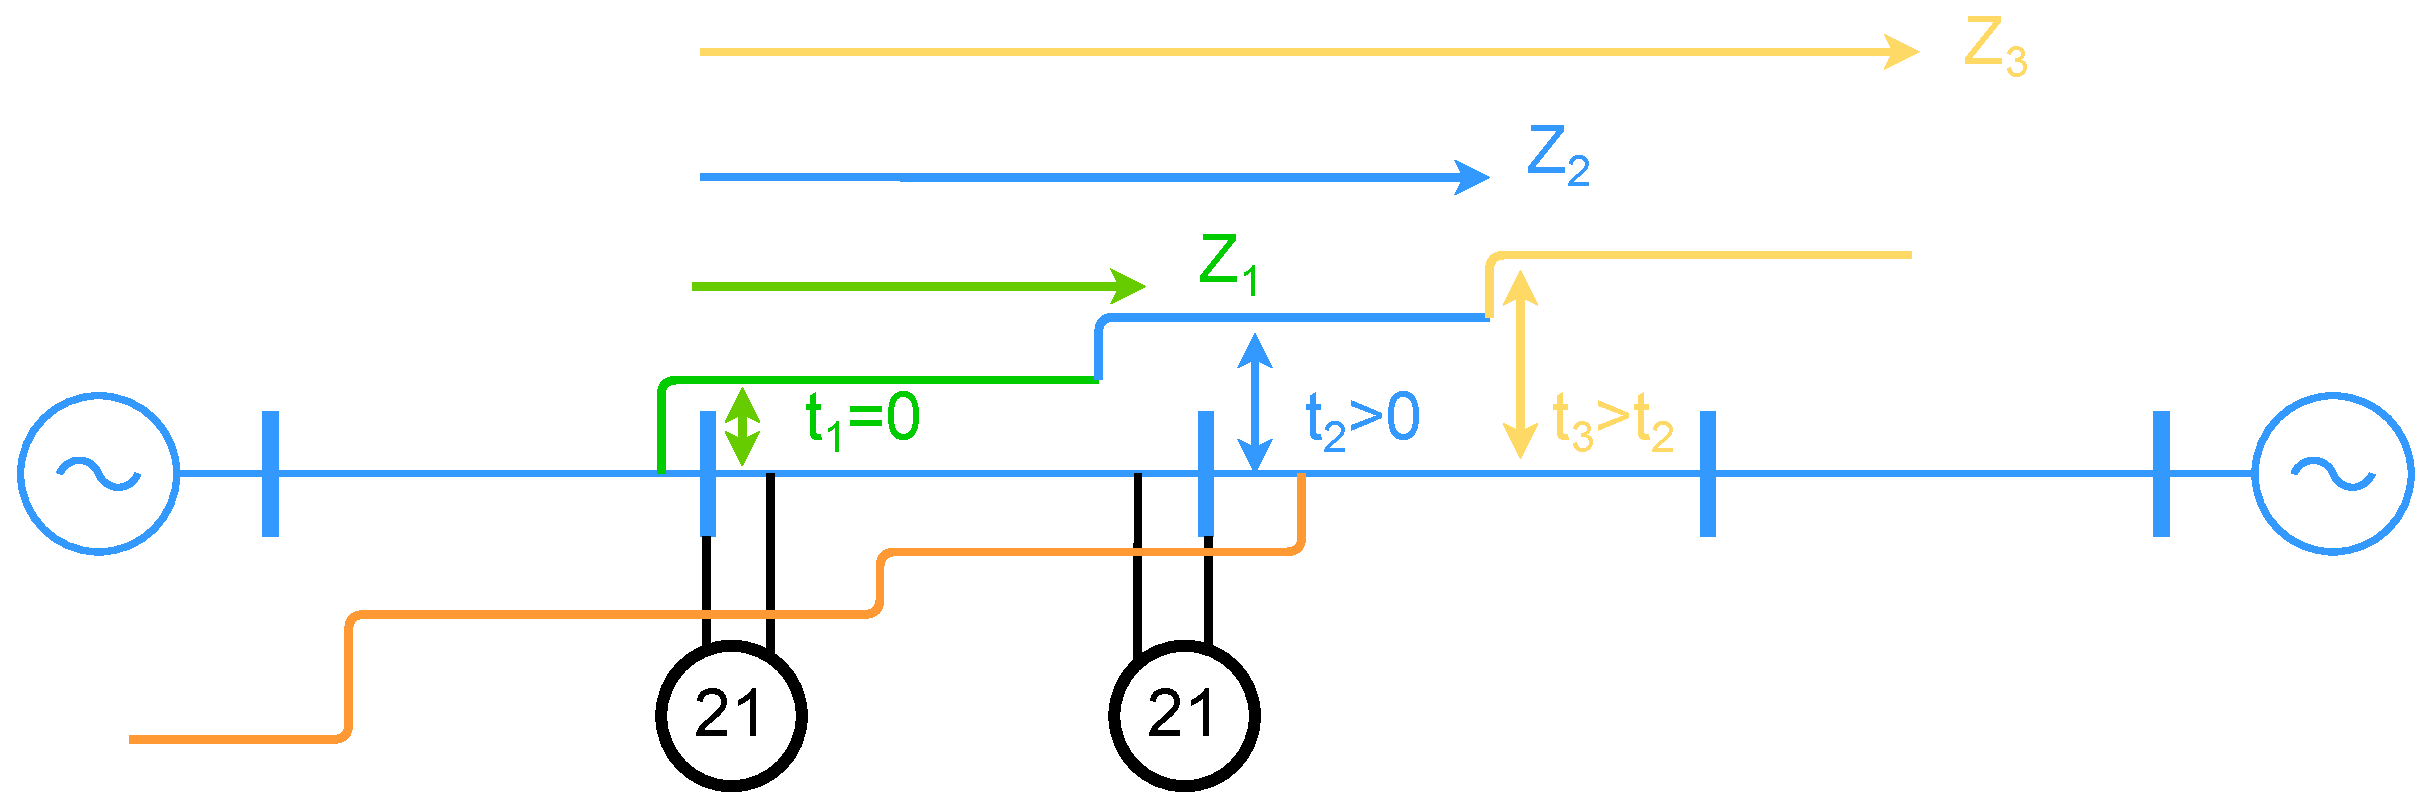
\includegraphics[width=1\textwidth]{shema5}
  \caption{Zone zaštite linija}
  \label{fig:shema5}
\end{figure}

\section{Proradne karakteristike distantnog releja}

Proradna karakteristika releja prikazuje se u ravni ${R,X}$. Cilj je izračunati impedansu kvara i ukoliko ona pripada zoni prorade koja je određena oblikom proradne karakteristike releja, znamo da je došlo do kvara. Bitno je da je proradna karakteristika odabrana u skladu sa zonom koju štiti, tj. sa područjem koje pokriva. To znači da je \textbf{potrebno poznavati karakteristike, tj. parametre mreže u režimu rada bez kvara}. 

U svakoj fazi evolucije dizajna distantnih releja razvoj oblika proradnih impedantnih karakteristika ovisi o dostupnoj tehnologiji i prihvatljivim troškovima.

Postoji nekoliko poznatih i danas korištenih proradnih karakteristika releja. Najjednostavniji releji su impedantni releji koji mjere odnos napona i struje neovisno o njihovom faznom položaju. To su tradicionalni releji koji mjere apsolutni odnos napona i struje te proračunavaju impedansu. Karakteristika ovakvih releja je kružnica sa središtem u koordinatnom početku ${R,X}$ čiji promjer odgovara proradnoj vrijednosti odgovarajuće zone releja. Obzirom da proradna vrijednost ne zavisi o uglu, relej bi djelovao i u slučaju kvara u suprotnom smjeru zaštite (treći kvadrant). Upravo zbog ovoga, relej ima poseban član koji je zadužen za smjer, a čija je karakteristika prikazana pravcem koji dijeli kružnicu na dva dijela i koji je okomit na impedansu voda. Slikom \ref{fig:slika1} prikazana je proradna karakteristika ovakvih releja. 

\begin{figure}[H]
  \centering
  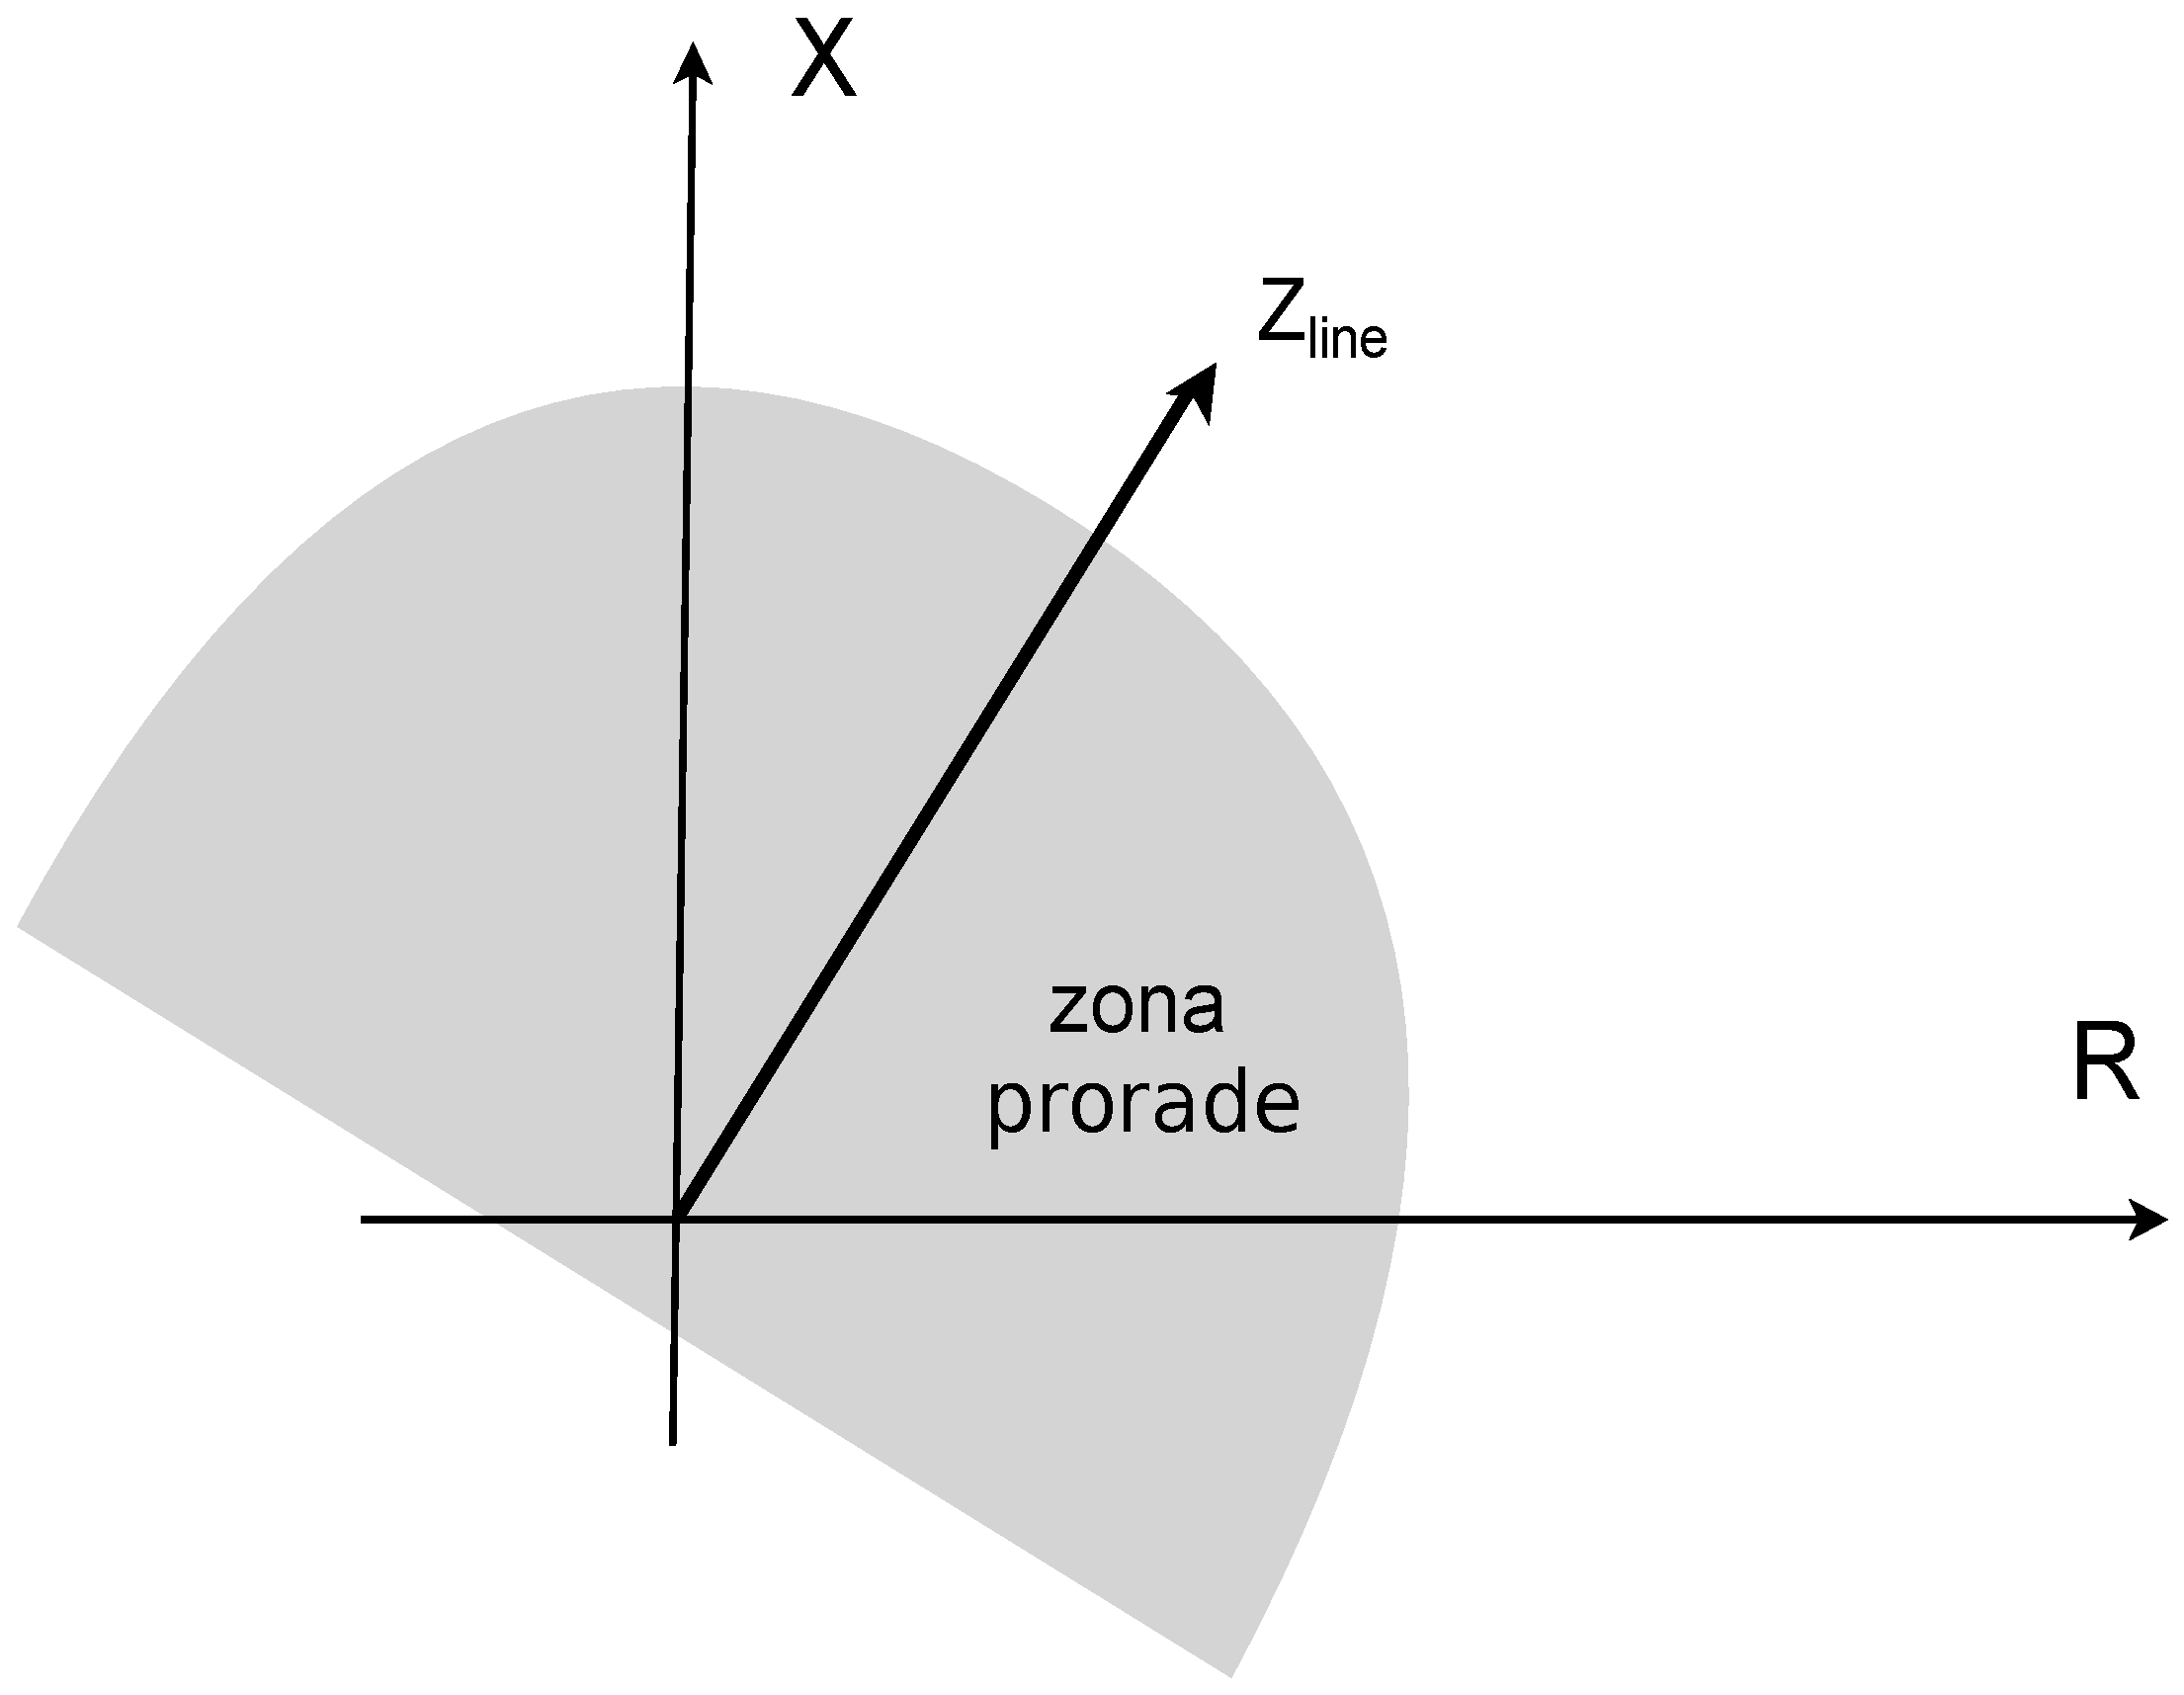
\includegraphics[width=0.6\textwidth]{slika1}
  \caption{Proradna karakteristika jednostavnog impedatnog releja}
  \label{fig:slika1}
\end{figure}

U praksi se često upotrebljavaju i distantni releji koji ne mjere direktno impedansu, nego mjere vodljivost štićene linije. Ovakvi releji nazivaju se inverzni impedantni releji ili Mho releji. Karakteristika prorade ovakvih releja može se predstaviti jednačinom:

\[\frac{1}{Z_rcos(\phi_r-\alpha)}\]

što u kompleksnoj ravni prestavlja kružnicu pomjerenu iz koordinatnog početka čiji centar zaklapa ugao $\alpha$ sa R osom. Kružnica prolazi kroz koordinatni početak i relej djeluje usmjereno. Slikom \ref{fig:slika2} prikazana je proradna karakteristika Mho releja. \cite{prva}

\begin{figure}[H]
  \centering
  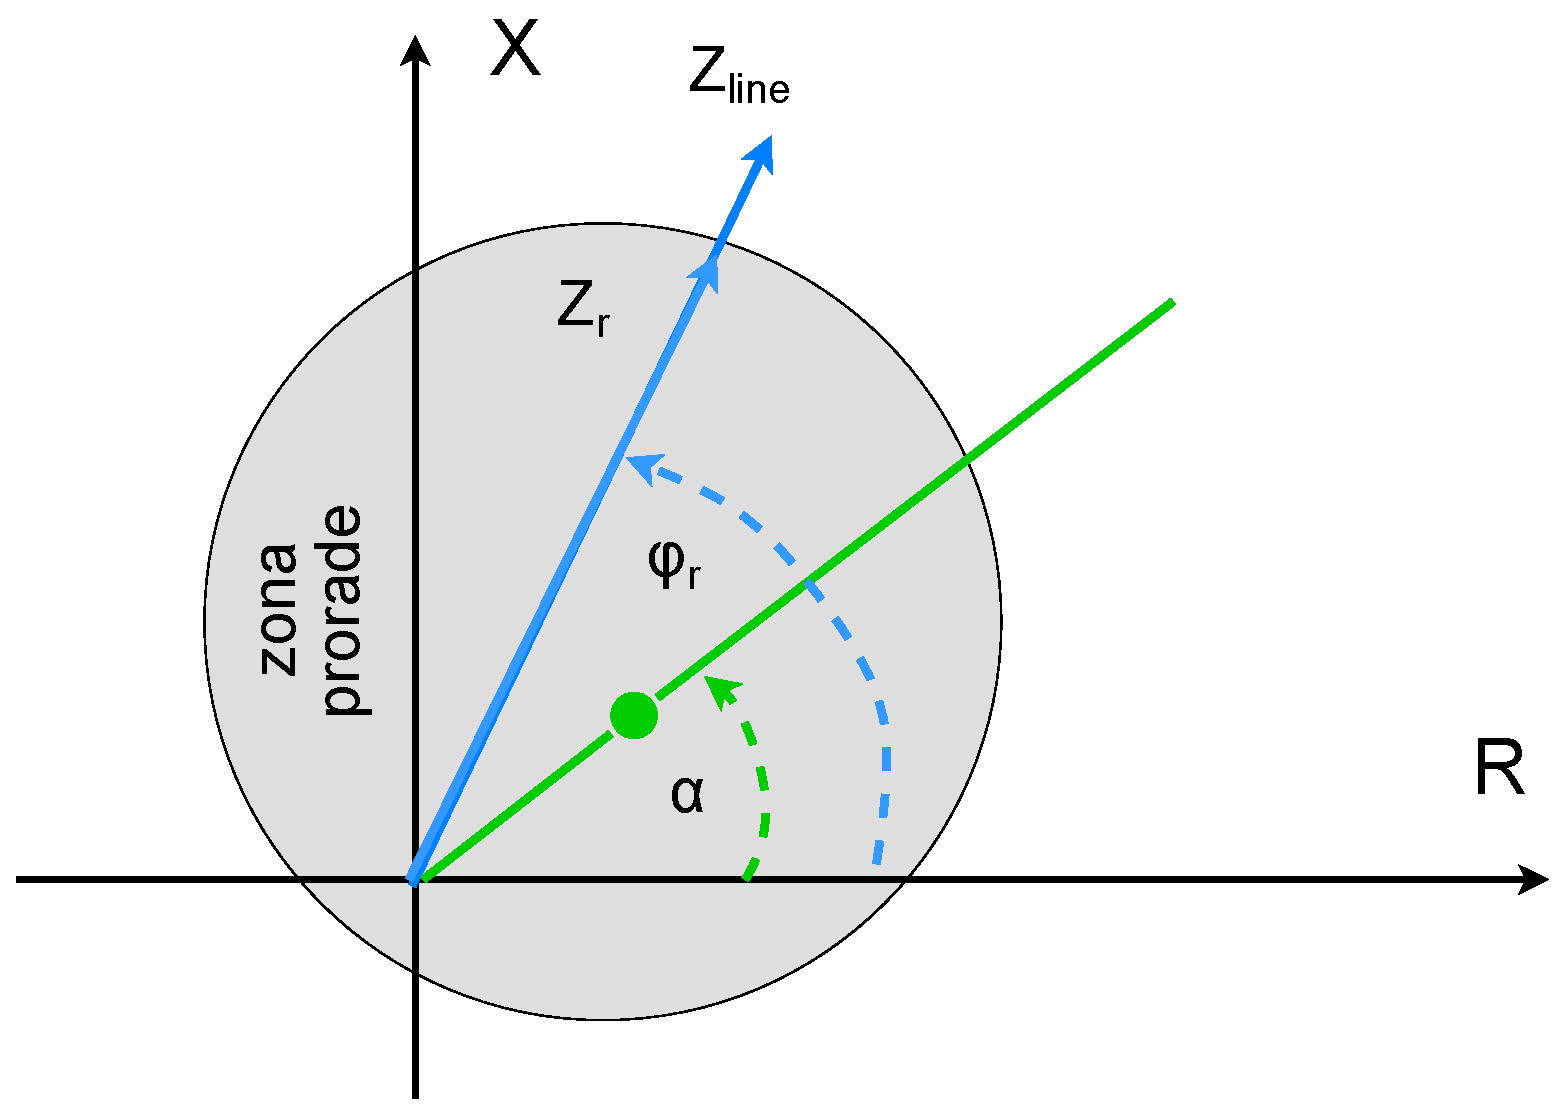
\includegraphics[width=0.6\textwidth]{slika2}
  \caption{Inverzno-impedantna karakteristika Mho releja}
  \label{fig:slika2}
\end{figure}

U ovom radu korištena je poligonalna impedantna karakteristika.

\subsection{Poligonalna karakteristika}
\label{poligon}

Kako bi se postigla što bolja karakteristika impedantnih releja razvijene su poligonalne karakteristike korištenjem usmjerenih i rezistantnih članova te se mogu idealno prilagoditi uvjetima zaštite. Ove karakteristike koriste se najčešće za zaštitu od zemljospoja na vodovima male i srednje duljine sa jakim izvorima gdje je potreban visok stupanj tolerancije za rezistanciju kvara. Nezavisno postavljanje četverostranih granica zone u R i X smjeru (poligonalna, tj. kvadrilateralna karakteristika) je izrazita prednost, jer je uvijek moguće postići dovoljno veliko pokrivanje otporu luka.  \cite{druga}

Da bismo kreirali poligonalnu karakteristiku potrebno je unijeti četri tačke koje predstavljaju koordinate u ${R, X}$ ravni, ali treba voditi računa na koji način biramo vrijednosti tih koordinata. Za početak, testiramo mrežu bez kvara da bi se odredili opsezi impedansi u normalnom radu gdje dodajemo i određen opseg tolerancije u kojem zaštita ne bi trebala da djeluje. Na osnovu izabranih koordinata računamo pravce koji će formirati našu poligonalnu karakteristiku. Ove pravce dobivamo pomoću standardne jednačine pravca: $y=kx+n$ na osnovu kojih računamo nagib i odsječak na $y$ osi za svaki pravac. Računajući impedansu za svaku fazu poredimo da li impedanse upadaju u poligonalnu zonu zaštite. Da bi se relej za posmatranu fazu aktivirao moraju biti zadovoljeni sljedeći uvjeti:

\begin{itemize}
    \item Impedansa faze mora ležati iznad pravca kojeg čine $Z_1$ i $Z_2$
    \item Impedansa faze mora ležati ispod pravca kojeg čine $Z_3$ i $Z_4$
    \item Impedansa faze mora ležati iznad pravca kojeg čine $Z_2$ i $Z_3$ ako je $k_2 > 0$, a ispod ako je $k_2 < 0$
    \item Impedansa faze mora ležati iznad pravca kojeg čine $Z_4$ i $Z_1$ ako je $k_4 < 0$, a ispod ako je $k_4 > 0$
\end{itemize}

Slikom \ref{fig:poligonalna} prikazan je primjer poligonalne karakteristike. 

\begin{figure}[H]
  \centering
  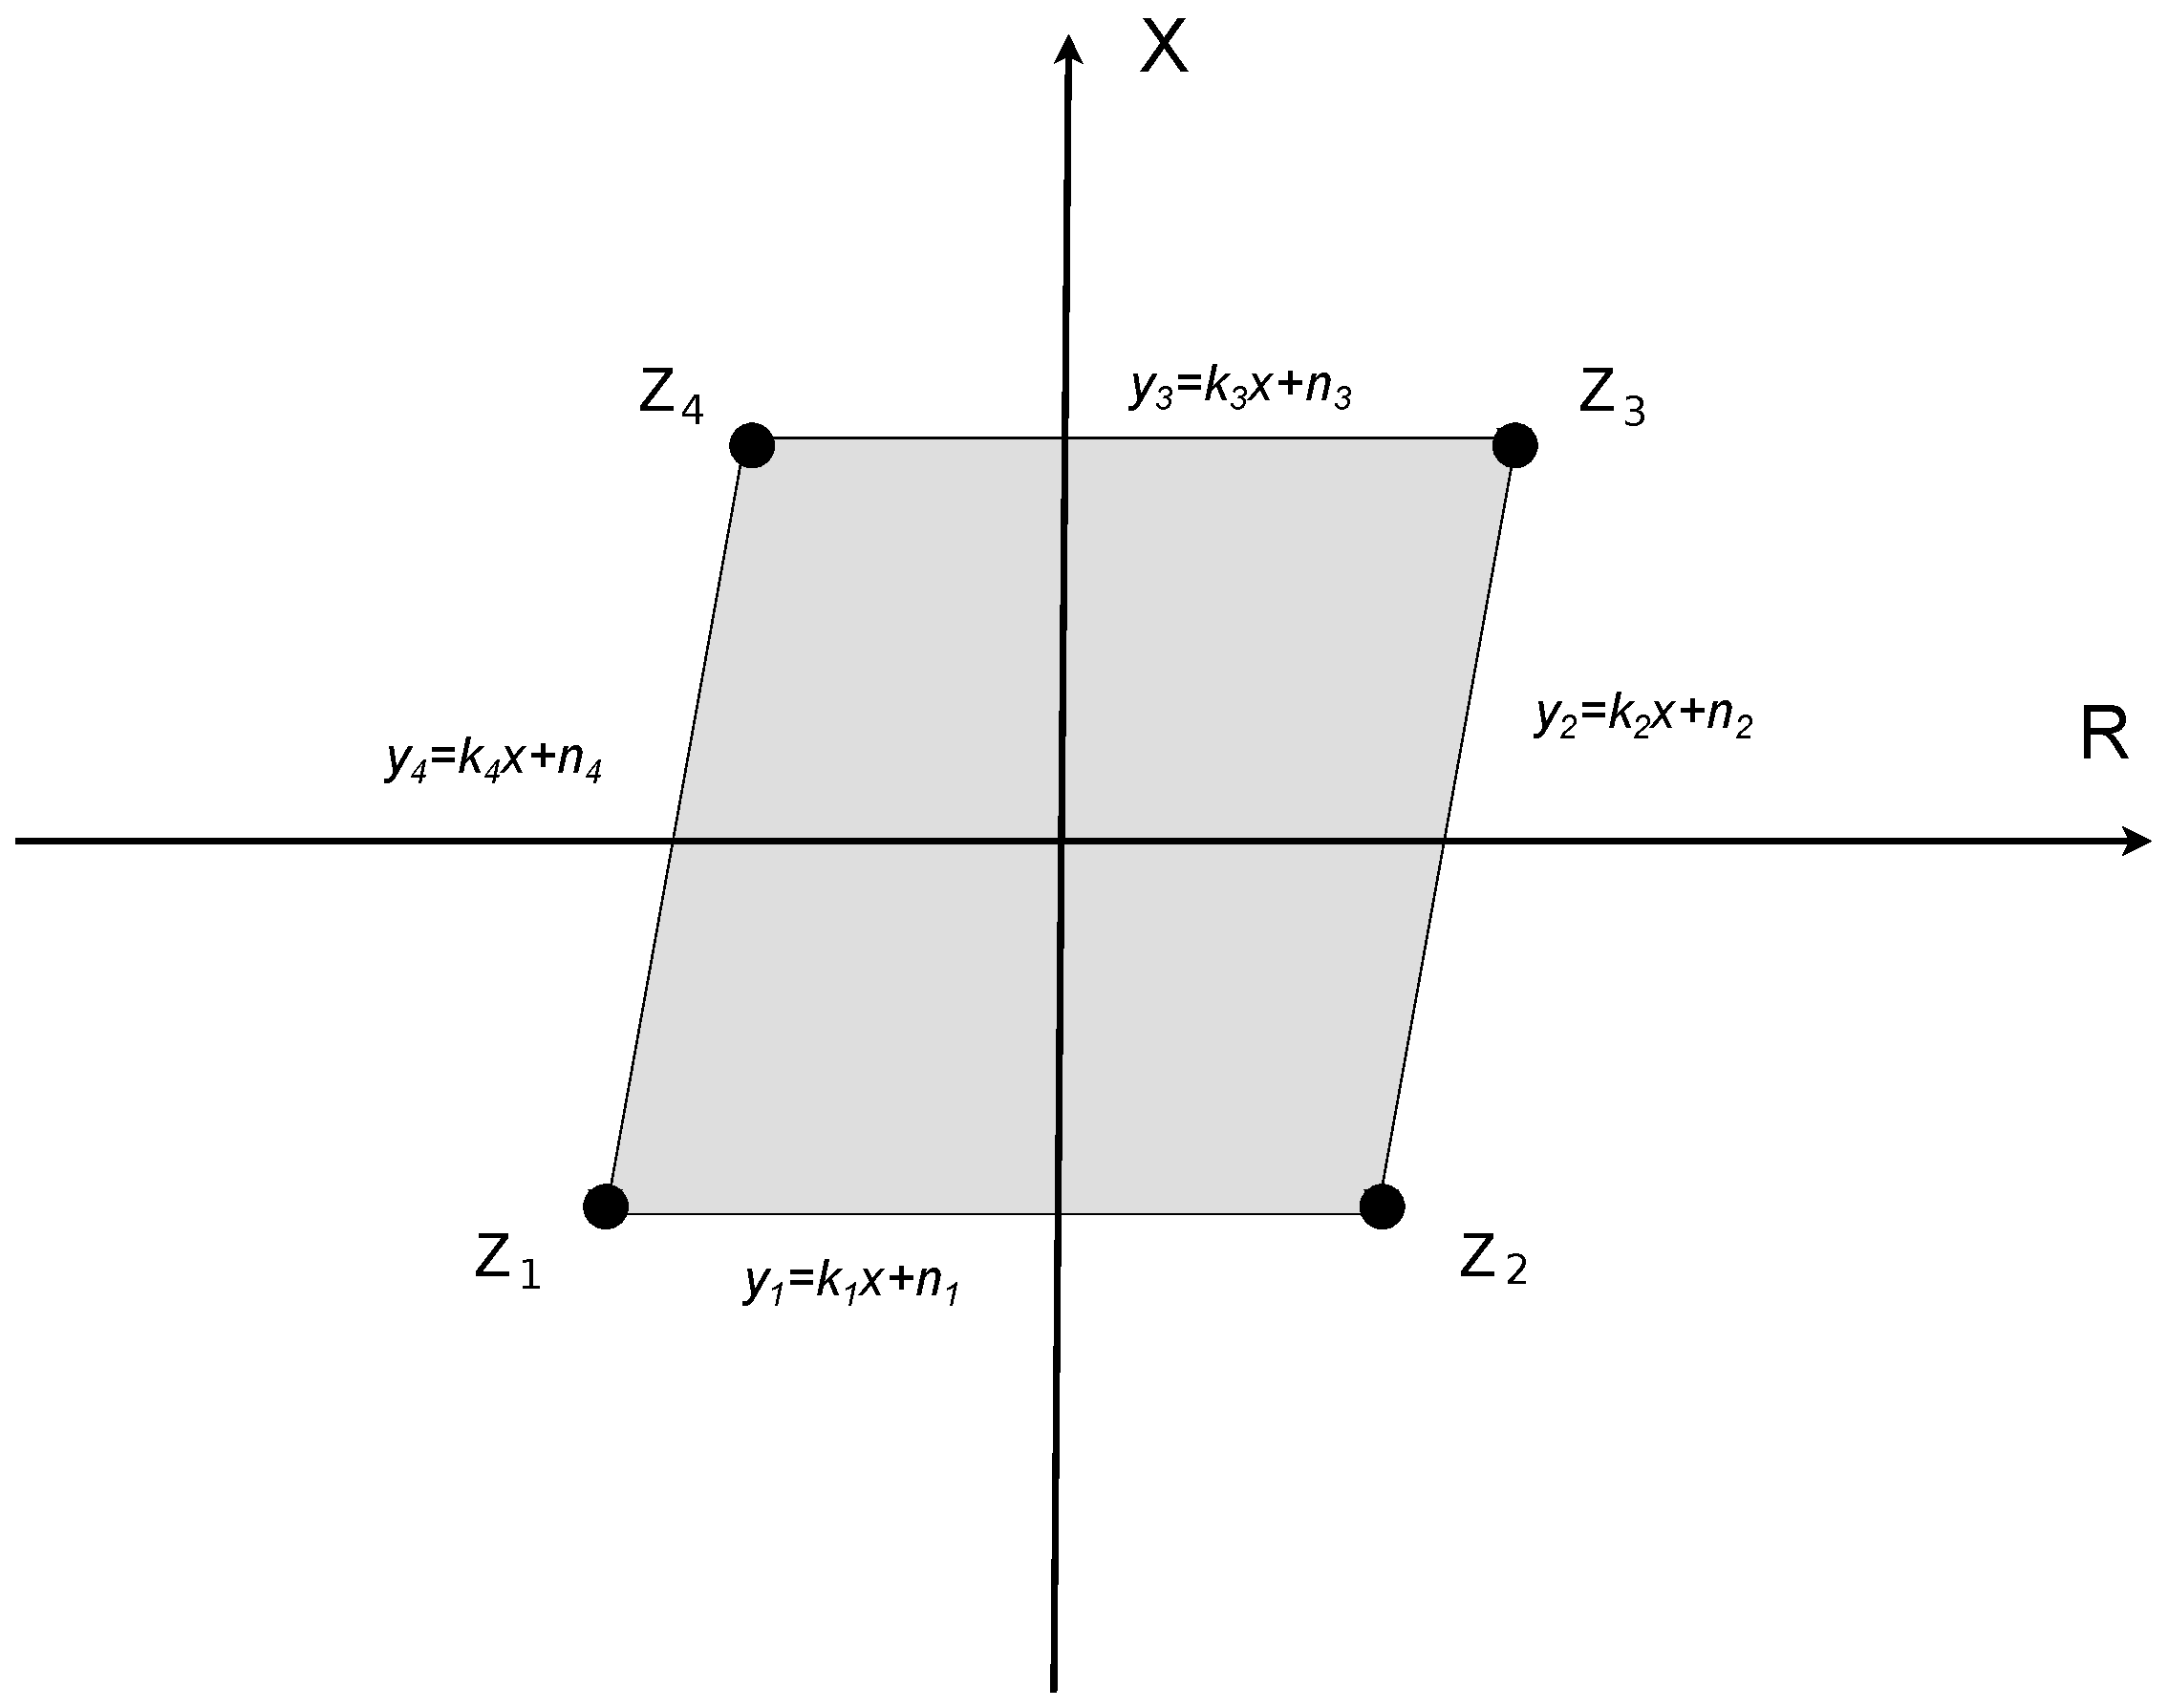
\includegraphics[width=0.9\textwidth]{poligonalna}
  \caption{Poligonalna karaktereistika}
  \label{fig:poligonalna}
\end{figure}

\section{Ekstrakcija fazora}

Da bi se mogla vršiti detekcija kvarova i generalno analiza ponašanja elektroenergetskog sistema potrebno je mjeriti određene veličine na određenim lokacijama u sistemu. Veličine koje se mjere su najčešće naponi i struje. Mjerenje se vrši u određenom vremenskom intervalu, a zatim se signali pretvaraju iz vremenskog u fazorski domen, a to se jednostavno može uraditi jer su signali u idealnom slučaju harmonijski. Relacijama \ref{eq:11} i \ref{eq:12} je prikazan signal \textit{x} u vremenskom i fazorskom domenu gdje se jasno vidi na koji način se prelazi iz jednog u drugi domen. Frekvencija na kojoj mreža radi je označena sa \textit{w}. 

\begin{equation}
    x(t) = \sqrt{2}A \; sin(wt+\phi)
    \label{eq:11}
\end{equation}

\begin{equation}
    X = A \; e^{j\phi}
    \label{eq:12}
\end{equation}

Problem nastaje iz razloga što signali koji se mjere nisu nikada idealnog harmonijskog oblika, već sadrže smetnje koje mogu nastati iz različitih razloga. Prva smetnja je nemogućnost izvedbe idealnog sinusnog signala, pa se pored fundamentalne komponente pojavljuju i viši harmonici sa frekvencijama koje predstavljaju cjelobrojni umnožak fundamentalne frekvencije. U praksi, sa porastom harmonika opada njihova amplituda što je bitna osobina u analizi signala. Druga smetnja je DC (istosmjerna) komponenta signala koja se pojavljuje uslijed prelaznog procesa prilikom kvara ili zbog zasićenja strujnih transformatora. Pored ovih smetnji javljaju se različiti tipovi šumova koji nastaju zbog mjerenja, AD konverzije, elektronskih sklopova, itd. Zadatak je da se iz mjerenog signala ekstraktuje fazor fundamentalne komponente, a da se smetnje filtriraju. Za to postoje različite metode koje imaju svoje prednosti i mane, a u ovom radu je prezentovana \textbf{metoda najmanjih kvadrata} u literaturi poznata kao \textbf{least squares method (LSM)}.  

\subsection{Metoda najmanjih kvadrata}

Razmotrimo statički proces kod kojeg je preslikavanje ulaza na izlaz nelinearno. Bez obzira na to, pretpostavka je da je izlaz linearno zavisan od parametara procesa, tj. kažemo da je takav proces "linearan po parametrima". Konkretno, izlaz u ovisnosti o parametrima možemo predstaviti kao:


\begin{equation}
    x(t)=K_0+u_1(t)K_1+u_2(t)K_2+...+u_q(t)K_q=K_0+\sum_{j=1}^{q} u_jK_j
\end{equation}

Pretpostavimo da je ulazna veličina $u(t)$ poznata. Ukoliko se na mjereni izlaz superponira smetnja $n(t)$, tada je izlazni signal dat sa:

\begin{equation}
    x(t)=x_u(t)+n(t)
\end{equation}

U svrhu analize ovog slučaja, korisno je formirati određene vektore i matrice koje su u skladu sa poznatom notacijom postavljenog problema. Kako su mjereni podaci diskretni, umjesto kontinualnog vremena \textit{t} se koristi \textit{$kT_s$}, gdje su:

\begin{itemize}
    \item \textbf{k} - redni broj uzorka, k = 1, 2, ... N (N je ukupan broj uzoraka)
    \item \textbf{$T_s$} - period uzorkovanja signala (pošto je period uzorkovanja konstantan, razmatrat ćemo samo ovisnost o k).
\end{itemize}

Slikom \ref{fig:LS} ilustrativno su prikazane veličine koje su korištene u izvođenju metode najmanjih kvadrata.

\begin{figure}[H]
  \centering
  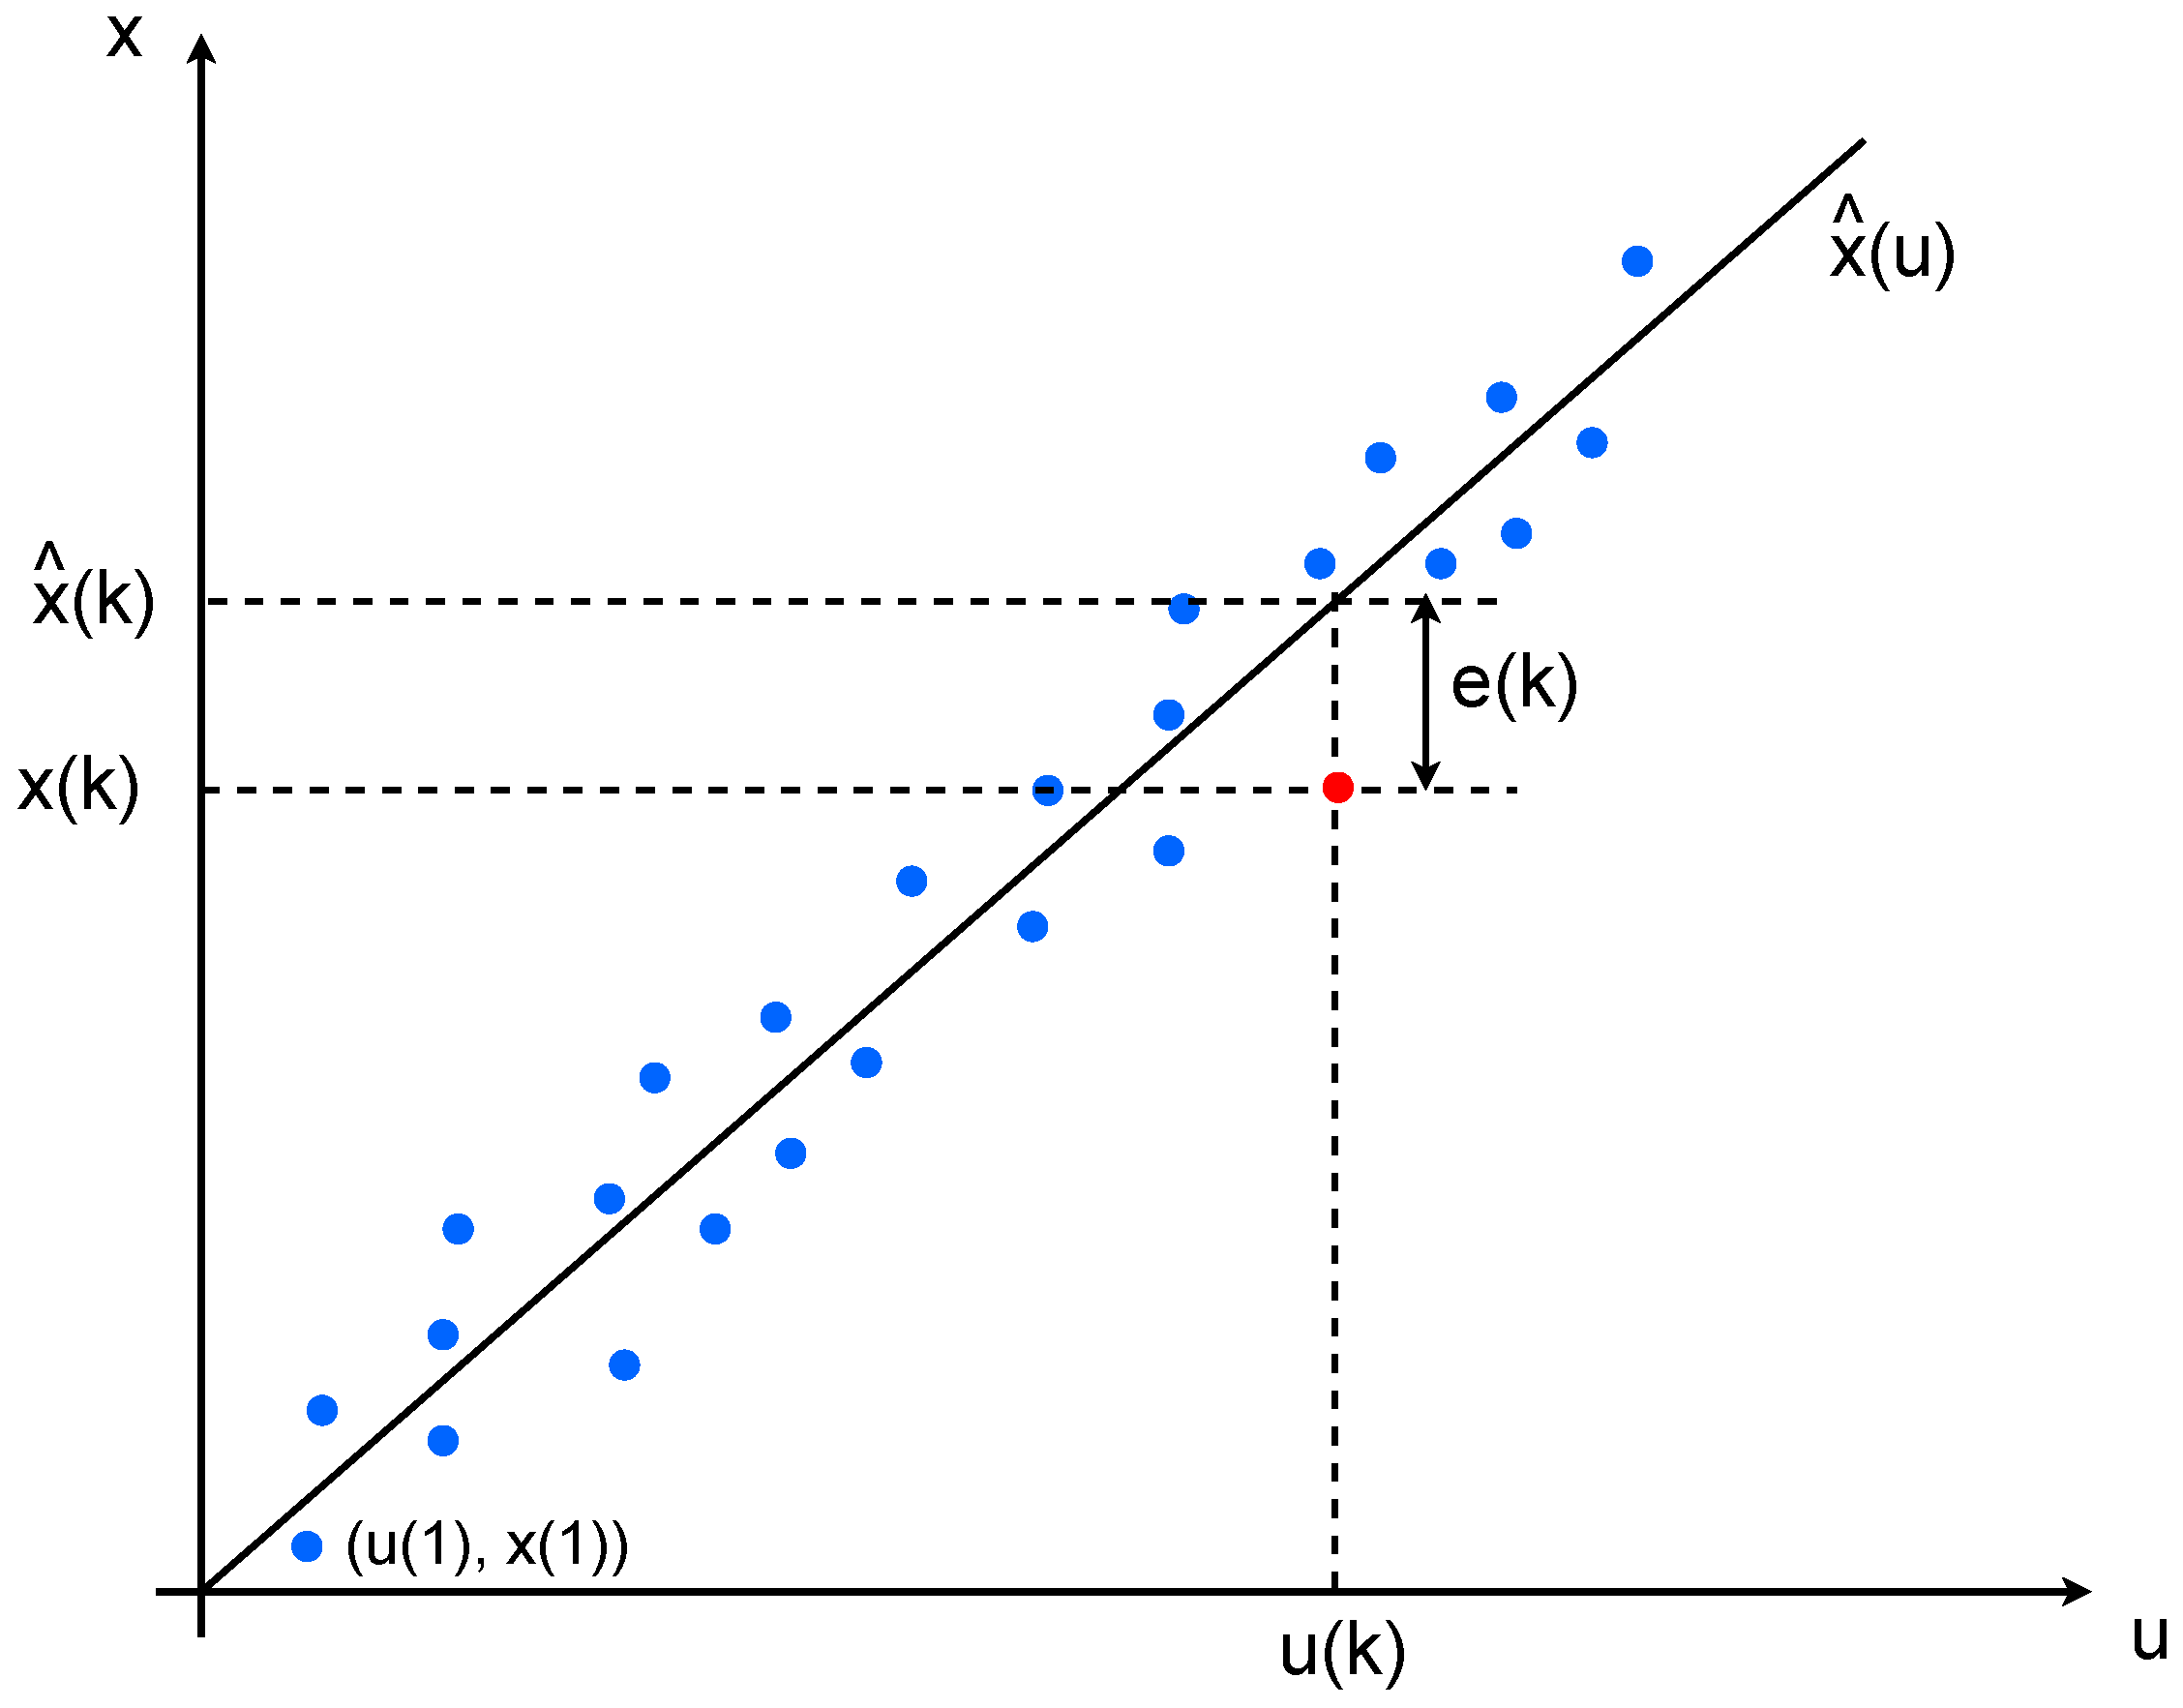
\includegraphics[width=0.7\textwidth]{LS}
  \caption{Metoda najmanjih kvadrata}
  \label{fig:LS}
\end{figure}

Matrica podataka imat će sljedeću formu:

\begin{equation}
    \Psi=\begin{pmatrix}
    1 & U_1(1) & U_2(1) & ... & U_q(1) \\
    1 & U_1(2) & U_2(2) & ... & U_q(2) \\
    . & . & . & ... & . \\
    1 & U_1(N) & U_2(N) & ... & U_q(N)
    \end{pmatrix}
\end{equation}

Vektor izlaza dat je kao: 

\begin{equation}
x= \begin{pmatrix}
    X(1)& X(2)& ... &X(N) 
\end{pmatrix}^T
\end{equation}

Vektor greške:
\begin{equation}
    e=\begin{pmatrix}
    e(1)& e(2)& ...& e(N) 
    \end{pmatrix}^T
\end{equation}

Vektor smetnje:
\begin{equation}
    n=\begin{pmatrix}
    n(1)& n(2)& ... &n(N) 
    \end{pmatrix}^T
\end{equation}

Vektor parametara:
\begin{equation}
    \Theta=\begin{pmatrix}
    K_0 & K_1 & ...& K_q 
    \end{pmatrix}^T
\end{equation}

Jednačinu procesa sada možemo napisati u jednostavnoj matričnoj formi:

\begin{equation}
   x=\Psi \Theta_0 +n
\end{equation}

Vektor $\Phi_0$ predstavlja stvarne (ali nepoznate) parametre procesa. Jednačinu modela možemo napisati kao: 

\begin{equation}
    \hat{x}=\Psi \Theta
\end{equation}

gdje je $\hat{x}$ izlaz, tj. pretpostavka modela. 

Izlaze modela i procesa možemno porediti sa ciljem formiranja izraza za grešku:

\begin{equation}
    e=x-\Psi \Theta
\end{equation}

Funkcija "cijene" data je kao:

\begin{equation}
    V=e^Te=(x^T-\Theta ^T \Psi ^T)(x-\Psi \Theta) 
\end{equation}
 tj.
 
\begin{equation}
    V=x^Tx - \Theta ^T \Psi ^Tx - (\Psi ^T x)^T \Theta + \Theta ^T \Psi ^T \Psi \Theta
\end{equation}

Primjenjujući pravila za derivaciju iz matrične analize imamo:

\begin{equation}
    \frac{d}{d\Theta}(\Theta ^T \Psi ^T x)=\Psi ^T x
\end{equation}

\begin{equation}
    \frac{d}{d\Theta}((\Psi ^T x)^T \Theta)=\Psi ^T x
\end{equation}

\begin{equation}
    \frac{d}{d\Theta}(\Theta ^T \Psi ^T \Theta \Psi)=2 \Psi ^T \Psi \Theta
\end{equation}

Derivaciju funkcije cijene po vektoru parametara sada možemo dobiti u obliku: 

\begin{equation}
    \frac{dV}{d\Theta}=-2\Psi ^Tx + 2\Psi ^T \Psi \Theta = -2 \Psi ^T (x- \Psi \Theta)
\end{equation}

Potreban uslov da bismo dobili optimum je (uzimamo da je $\Theta=\hat{\Theta}$): 

\begin{equation}
    \frac{dV}{d\Theta} = 0
\end{equation}

Iz posljednje dvije relacije rješenje problema estimacije možemo prikazati u obliku: 

\begin{equation}
    \hat{\Theta}=(\Psi ^T \Psi)^{-1} \Psi ^T x
    \label{eq:lsm}
\end{equation}

Potrebno je da matrica $\Psi ^T \Psi$ ne bude singularna kako bi egzistiralo rješenje posljednje jednačine, tj. treba da vrijedi:

\begin{equation}
    det(\Psi ^T \Psi) \neq 0
\end{equation}

Očekivana vrijednost  estimacije vektora parametara data je sa:

\begin{equation}
    E\{\hat{\Theta}\}= \Theta + E \{(\Psi ^T \Psi) ^{-1} \Psi ^T n\} = \Theta
\end{equation}

Treba napomenuti da je implicitno pretpostavljeno da elementi matrice podataka i elementi vektora šuma nisu korelisani, te da je $E\{n(k)\}=0$. U ovom slučaju estimacija nije pristrasna. Zaključak je da su parametri nelinearnog statičkog procesa estimirani konzistentno u smislu srednje kvadratne greške ukoliko su zadovoljeni uslovi: 
\begin{itemize}
    \item ulazni signal U(k) je direktno mjerljiv
    \item vrijedi da je $det(\Psi ^T \Psi) \neq 0$
    \item smetnja je stacionarna i estimirana vrijednost smetnje je $E\{n(k)\}=0$
    \item ulazna veličina U(k) je nekorelisana sa smetnjom n(k). \cite{treca}
\end{itemize} 

\vspace{0.5cm}
\begin{center}
    * * *
\end{center}

\vspace{0.5cm}

Razmotrimo sada primjenu opisane metode za potrebe rješavanja problema ekstrakcije fazora. Mjereni signal se može prepostaviti u sljedećem obliku:

\begin{equation}
    x(t) = B_0\;e^{-dt} + \sum_{n=1}^{M} B_n\;sin(nwt+\phi_n) + sh(t)  
    \label{eq:13}
\end{equation}

gdje su:

\begin{itemize}
    \item $B_0\;e^{-dt}$ - DC komponenta
    \item $\sum_{n=1}^{M} B_n\;sin(nwt+\phi_n)$ - fundamentalna komponenta (n=1) i viši harmonici (n>1) 
    \item $sh(t)$ -  ostali šumovi
\end{itemize}

Šumovi koji djeluju na signal su obično u obliku Gaussovog bijelog šuma čija je srednja vrijednost nula. Metoda najmanjih kvadrata traži krivu koja najbolje opisuje sve posmatrane tačke u smislu kvadratne greške, a za bijeli šum sa srednjom vrijednošću nula to je zapravo pravac sa koeficijentom i offsetom jednakim nuli, pa se ova metoda inherentno dobro nosi sa ovakvim šumom, te ga možemo izostaviti iz daljne analize koja je bazirana na radu \cite{LSmetoda}. Osnovna mana ove metode je što se loše nosi sa velikim vrijednostima parametra \textbf{d} kod DC komponente. LS metoda se može primijeniti na funkcije koje su linearne po parametrima, što nije slučaj kod DC komponente, pa se pristupa razvoju DC komponente u Taylorov red u okolini nule. Izraz \ref{eq:14} prikazuje razvoj sa prva tri člana, što je sasvim dovoljno. 

\begin{equation}
    B_0\;e^{-dt} \approx B_0 - B_0 d\;t + \frac{1}{2} B_0 d^2\;t^2 = K_1 + K_2\;t + K_3\;t^2 
    \label{eq:14}
\end{equation}

Fundamentalna komponenta se korištenjem trigonometrijskih identiteta može zapisati kao:

\begin{equation}
    B_1\;sin(wt+\phi_1) = B_1cos(\phi_1)\;sin(wt) + B_1sin(\phi_1)\;cos(wt) = K_4\;sin(wt) + K_5\;cos(wt)
    \label{eq:15}
\end{equation}

Na sličan način se mogu prikazati i viši harmonici, pa se mjereni signal na koji se primjenjuje LS metoda može prikazati izrazom \ref{eq:16}. 

\begin{equation}
    \begin{split}
    x(t) & = B_0 - B_0 d\;t + \frac{1}{2} B_0 d^2\;t^2 + B_1cos(\phi_1)\;sin(wt) + B_1sin(\phi_1)\;cos(wt) + \\ 
    & + B_2cos(\phi_2)\;sin(2wt) + B_2sin(\phi_2)\;cos(2wt) + ... \\ 
    & + B_Mcos(\phi_M)\;sin(Mwt) + B_Msin(\phi_M)\;cos(Mwt)
    \end{split}
    \label{eq:16}
\end{equation}

Iz izraza \ref{eq:16} se mogu formirati matrica podataka i vektor parametara, a kako su mjereni podaci diskretni umjesto kontinualnog vremena \textit{t} se koristi \textit{$kT_s$}, gdje su:

\begin{itemize}
    \item \textbf{k} - redni broj uzorka, k = 1, 2, ... N (N je ukupan broj uzoraka)
    \item \textbf{$T_s$} - period uzorkovanja signala
\end{itemize}
\begin{equation}
\scalebox{0.89}{$\Psi = 
    \begin{pmatrix}
    1 & T_s  & {T_s}^2    & sin(w(T_s))  & cos(w(T_s))  & ... & sin((Mw)(T_s))  & cos((Mw)(T_s))  \\
    1 & 2T_s & {(2T_s)}^2 & sin(w(2T_s)) & cos(w(2T_s)) & ... & sin((Mw)(2T_s)) & cos((Mw)(2T_s)) \\
    1 & 3T_s & {(3T_s)}^2 & sin(w(3T_s)) & cos(w(3T_s)) & ... & sin((Mw)(3T_s)) & cos((Mw)(3T_s)) \\
    . & .      & .            & .              & .              & ... & .                 & .                 \\
    . & .      & .            & .              & .              & ... & .                 & .                 \\
    1 & NT_s & {(NT_s)}^2 & sin(w(NT_s)) & cos(w(NT_s)) & ... & sin((Mw)(NT_s)) & cos((Mw)(NT_s)) 
    \end{pmatrix}$}
\end{equation}
\\

\begin{equation}
    x^T = 
    \begin{pmatrix}
    x(1) & x(2)  & x(3)  & x(4)  & x(5)  & ... & x(N-1)  & x(N) 
    \end{pmatrix}
\end{equation}

\begin{equation}
{\Theta}^T = 
    \begin{pmatrix}
    B_0 & -B_0d  & \frac{1}{2} B_0 d^2  & B_1cos(\phi_1)  & B_1sin(\phi_1)  & ... & B_Mcos(\phi_M)  & B_Msin(\phi_M) 
    \end{pmatrix}
\end{equation}


Na osnovu matrice podataka $\Psi$ i mjerenog signala \textbf{x} se dobiju parametri $\Theta$ prema formuli \ref{eq:lsm} iz kojih se mogu dobiti amplitude i faze svih harmonika, kao i koeficijenti DC komponente. Od interesa je da se izvuku amplituda i faza fundamentalne kompnente, tj. $B_1$ i $\phi_1$. Oni se mogu prema onome kako je ovdje prikazano izvući iz 4. i 5. elementa vektora parametara, pa te elemente označimo sa $K_4$ i $K_5$.

Vrijedi da je:

\begin{equation}
    K_4 = B_1cos(\phi_1)
    \label{eq:17}
\end{equation}
\begin{equation}
    K_5 = B_1sin(\phi_1)
    \label{eq:18}
\end{equation}

Kombiniranjem jednačine \ref{eq:17} i \ref{eq:18} se jednostavno dobiju faza i amplituda fundamentalne komponente što je i bio početni cilj:

\begin{equation}
    \phi_1 = arctg\frac{K_5}{K_4}
    \label{eq:19}
\end{equation}

\begin{equation}
    B_1 = \frac{K_5}{sin(\phi_1)}
    \label{eq:110}
\end{equation}